\documentclass  [paper=a4,
				fontsize=12pt,
				listof=totoc,
				bibliography=totoc
				]{scrreprt}
\usepackage[T1]{fontenc}
\usepackage[utf8]{inputenc}
\usepackage{mathptmx}				%Font: Times New Roman
%\usepackage[default]{droidserif}	%Font: Droid Serif
\usepackage[ngerman]{babel}
%Seitenränder einstellen
\usepackage[head=2cm,bottom=2cm, left=25mm, right= 25mm ]{geometry}
%Paket für Erzeugung eines Abkürzungsverzeichnis, über das auch per Befehl im späteren Text auf diese verwiesen werden kann
\usepackage[printonlyused,smaller]{acronym}
%Paket zur Gestaltung der Kopf- und Fusszeile bei KOMA-Script
\usepackage{scrpage2}
\usepackage[hidelinks]{hyperref}
%Bibliograpie Packages / Settings
\usepackage{ragged2e} % Ermöglicht Flattersatz mit Silbentrennung
\usepackage[babel,german=guillemets]{csquotes}
% damit werden Zitate in französische Anführungszeichen gesetzt
\usepackage[%
backend=biber,% damit wird bestimmt, dass Sie mit der biber.exe arbeiten
bibencoding=utf8,% steht für die Kodierung der .bib-Datei
bibwarn=true,% damit werden ggf. enstandene Fehler ausgegeben
style=alphabetic,% hier wird die DIN 1505-T2 eingebunden
%firstinits=true% der Familienname des Authors wird an die erste Stelle
% gesetzt und anschließend der Vorname nur mit dem ersten
% Buchstaben abgekürzt ausgegeben
]{biblatex}
\usepackage[babel]{microtype} % bringt optischen Randausgleich und
% minimale Skalierung der Buchstaben
\setlength\bibitemsep{8pt} % Abstand zwischen 2 Einträgen im Verzeichnis
% nachfolgend wird der Kopf des Literaturverzeichnisses bestimmt
\defbibheading{online}{\subsection*{Online-Quellen}}
\defbibheading{offline}{\subsection*{Literatur}}
\ExecuteBibliographyOptions{
%isbn=false, % falls die ISBN hinterlegt ist wird diese ausgeblendet
}
\addbibresource{bibliothek.bib} % Einbindung der Literaturquelldatei
%Fortlaufende Fußnoten
\usepackage{chngcntr}
\counterwithout{footnote}{chapter}
%Paket zum Einbinden von Grafiken
\usepackage[pdftex]{graphicx}
\usepackage{wrapfig}
\usepackage{caption}


% Bibtexkey vor Quellenangabe (Jedoch nur bei stlye=alphabetic)
\DeclareFieldFormat{labelalpha}{\thefield{entrykey}}
\DeclareFieldFormat{extraalpha}{}

\usepackage{filecontents}
\usepackage{multicol}
\usepackage{relsize} %Einbinden der benötigten Pakete über die Datei Pakete.tex, wobei die Dateiendung weggelassen wird
\hyphenation{words} % LaTeX Wörter übergeben werden, die es entweder nicht selbstständig trennen kann(und hierdurch die entsprechenden Stellen markiert werden) oder nicht trennen soll\textbf{}
\counterwithout{figure}{chapter}
\counterwithout{table}{chapter} 
\begin{document}
	\parindent 0pt %entfernt den Einzug nach Absätzen
	%\begin{titlepage}
\begin{figure}
  \begin{center}
    \hbox to \hsize{%
      \begin{tabular}[m]{c}
        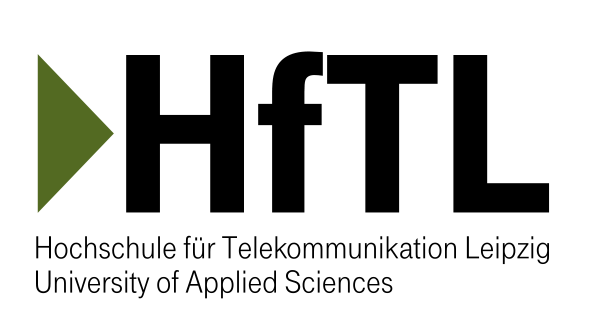
\includegraphics[width=2.5cm]{images/HfTL-Logo.png}
      \end{tabular}
      \hfill%
      \begin{tabular}[m]{c}
        Hochschule für Telekommunikation Leipzig (FH)\\
        Wirtschaftsinformatik \\
        Wissenschaftlich angeleitete Berufspraxis III\\
      \end{tabular}%
    }
  \end{center}
\end{figure}

\begin{center}
\rule{0pt}{0pt}
\vfill
\vfill
\vfill
\vfill

\begin{huge}
WAB III Projektarbeit:\\[0.75ex]
\dots\\[0.75ex]
E-Mail-Sicherheit\\[0.75ex]
\dots\\[0.75ex]
\end{huge}

\vfill
\vfill

Projektarbeit\\ von\\

\vspace*{.5cm}
Pascal Feller\\
Daniel Moy\\
Florian Schünhoff\\
Chi Cong Tran\\
\vspace{.5cm}
28. Juni 2014\\

\vfill
\vfill
\vfill
\vfill

\begin{tabular}{rl}
Referent, Betreuer:   & Prof. Dr. - Ing. Undine Pielot\\
\end{tabular}
\end{center}
\end{titlepage}



\newpage
\pagestyle{empty}


\text{ }
\vspace{11.5cm}




Hiermit versichern wir, dass wir die von uns vorgelegte Arbeit selbstständig verfasst haben, dass wir die verwendeten Quellen, Internet-Quellen und Hilfsmittel vollständig angegeben haben und dass wir die Stellen der Arbeit -- einschließlich Tabellen, Karten und Abbildungen~--, die anderen Werken oder dem Internet im Wortlaut oder dem Sinn nach entnommen sind, auf jeden Fall unter Angabe der Quelle als Entlehnung kenntlich gemacht haben.\\

Leipzig, den 28. Juni 2014\\
\medskip
\medskip

(Unterschrift)\\
\underline{~~~~~~~~~~~~~~~~~~~~~~~~~~~~~~~~~~~~~~~~}\\
Pascal Feller\\
\underline{~~~~~~~~~~~~~~~~~~~~~~~~~~~~~~~~~~~~~~~~}\\
Daniel Moy\\
\underline{~~~~~~~~~~~~~~~~~~~~~~~~~~~~~~~~~~~~~~~~}\\
Florian Schünhoff\\
\underline{~~~~~~~~~~~~~~~~~~~~~~~~~~~~~~~~~~~~~~~~}\\
Chi Cong Tran\\

\newpage


	\pagestyle{empty} %\pagestyle{empty} sorgt dafür, das keine Seitenzahl auf der entsprechenden Seite auftaucht
	\pagebreak	%Seitenumbruch
	\pagenumbering{Roman}
	\tableofcontents %Inhaltsverzeichnis		
	\pagebreak
	\listoffigures %Abbildungsverzeichnis
	\pagebreak
	\listoftables %Tabellenverzeichnis
	\pagebreak
	\phantomsection \addcontentsline{toc}{chapter}{Abkürzungsverzeichnis}
\renewcommand\refname{Abkürzungsverzeichnis} \chapter*{Abkürzungsverzeichnis}
\begin{acronym}[StuRa] % In die optionale eckige Klammer die längste Abkürzung schreiben (für gemeinsame Ausrichtung)
	\acro{DHE}{Diffie-Hellmann-Verfahren}
	\acro{TLS/SSL}{Transport Layer Security/Secure Socket Layer}
	\acro{PFS}{Perfect Foreward Secrecy}
\end{acronym} %einbinden des in Akronyme.tex erstellten Abbildungsverzeichnisses
	\pagebreak
	\pagenumbering{arabic}\setcounter{page}{1} %ändern der Seitennummerierung auf arabische Zahlen und Beginn bei Seite 1
	%%Dies ist die Vorlage für die einzelnen Kapitel, die jeweils mit Chapter als Kapiteltitel starten
\chapter{Titel des Kapitels}

%mit \section{title} wird ein Unterkapitel der ersten Gliederungsebene überschrieben
\section{Wichtiges Unterkapitel erster Gliederungsebene}
Lorem ipsum \dots

%mit \subsection{title} wird ein Unterkapitel der zweiten Gliederungsebene überschrieben
\subsection{Wichtiges Unterkapitel der zweiten Gliederungsebene}
Lorem ipsum \dots

%Vom Grundsatz war es das für die Erstellung von Kapiteln, jetzt kommt noch ein kleines Beispiel für Fußnoten
Dies ist ein großartiges Beispiel \footnote{Wenn einem nix einfällt muss man eben Quatsch schreiben} für eine Fußnote.
	%%Dies ist die Vorlage für die einzelnen Kapitel, die jeweils mit Chapter als Kapiteltitel starten
\chapter{Datensicherheit 1x1}
Unter Datensicherheit wird der Schutz von Daten in den Aspekten Verfügbarkeit, Vertraulichkeit und Integrität verstanden. \footnote(https://www.bsi.bund.de/DE/Themen/ITGrundschutz/ITGrundschutzKataloge/Inhalt/Glossar/glossar_node.html). Im Gegensatz dazu beschreibt Datenschutz den Schutz von und den vertrauensvollen Umgang mit persönlichen Daten. In der IT-Sicherheit wird zusätzlich des Aspekt der Authentizität berücksichtigt \footnote{http://www.datenschutz-berlin.de/content/technik/begriffsbestimmungen/verfuegbarkeit-integritaet-vertraulichkeit-authentizitaet}. In diesem Abschnitt werden diese Aspekte näher betrachtet, da diese für das Verstädnis der vorgestellten Techniken in den späteren Kapitel notwendig sind.

%mit \section{title} wird ein Unterkapitel der ersten Gliederungsebene überschrieben
\section{Verfügbarkeit}

Unter Verfügbarkeit wird das Vorhandensein von Infrastruktur, Software, sämtliche IT-Dienstleistungen sowie -Funktionalitäten und Daten verstanden, so dass die Anwender bei Bedarf darauf zugreifen und nutzen können. Um dies zu gewährleisten, muss verhindert werden, dass
\begin{itemize}
\item Daten verschwinden oder nicht zugreifbar sind, wenn sie gebraucht werden,
\item Programme nicht funktionsbereit sind, wenn sie aufgerufen werden sollen,
\item Hardware und sonstige notwendige Mittel nicht funktionsfähig oder gar verschwunden sind, wenn sie für die Verarbeitung benötigt wird. \footnote{http://www.datenschutz-berlin.de/content/technik/begriffsbestimmungen/verfuegbarkeit-integritaet-vertraulichkeit-authentizitaet}
\end{itemize}

\section{Integrität}
Unter der Integrität der Daten wird verstanden, dass die Daten nicht ohne Aufzufallen verändert werden können und somit vollständig übermittelt worden sind. Bei diesem Aspekt geht es demzufolge um die Unversehrtheit der Nachricht.

\section{Vertraulichkeit}

Unter Vertraulichkeit versteht man den Schutz der Nachricht vor unbefugtem Zugriff durch Dritte. Nur der gewünschte Empfänger soll in der Lage sein, den Inhalt der Nachricht zu erfahren. Dazu werden mathematische Verfahren genutzt, die in den späteren Kapiteln behandelt werden.

\section{Authentizität}

Bei der Authentizität geht es darum, nachzuweisen, dass die beteiligten Kommunikationspartner tatsächlich diejenigen sind, für die sie sich ausgeben.
	\chapter*{Selbstständigkeitserklärung}
	\chapter{Einleitung}
		\section{Motivation}
		\section{Zielsetzung und Zielperspektive}
		\section{Abgrenzung}
		%evtl. unnötig wenn Zielsetzung klar formuliert

	%Dies ist die Vorlage für die einzelnen Kapitel, die jeweils mit Chapter als Kapiteltitel starten
	\chapter{Datensicherheit Einmaleins}
	Unter Datensicherheit wird der Schutz von Daten in den Aspekten Verfügbarkeit, Vertraulichkeit und Integrität verstanden. \footcite{BSI2014} Im Gegensatz dazu beschreibt Datenschutz den Schutz von und den vertrauensvollen Umgang mit persönlichen Daten. In der IT-Sicherheit wird zusätzlich des Aspekt der Authentizität berücksichtigt \footcite{Berliner2014}. In diesem Abschnitt werden diese Aspekte näher betrachtet, da diese für das Verständnis der vorgestellten Techniken in den späteren Kapitel notwendig sind.
	
	%mit \section{title} wird ein Unterkapitel der ersten Gliederungsebene überschrieben
	\paragraph{Verfügbarkeit}
	
	Unter Verfügbarkeit wird das Vorhandensein von Infrastruktur, Software, sämtliche IT-Dienstleistungen sowie -Funktionalitäten und Daten verstanden, so dass die Anwender bei Bedarf darauf zugreifen und nutzen können. Um dies zu gewährleisten, muss verhindert werden, dass
	\begin{itemize}
	\item Daten verschwinden oder nicht zugreifbar sind, wenn sie gebraucht werden,
	\item Programme nicht funktionsbereit sind, wenn sie aufgerufen werden sollen,
	\item Hardware und sonstige notwendige Mittel nicht funktionsfähig oder gar verschwunden sind, wenn sie für die Verarbeitung benötigt wird. \footcite{Berliner2014}
	\end{itemize}
	
	\paragraph{Integrität}
	Unter der Integrität der Daten wird verstanden, dass die Daten bei der Übertragung nicht unbemerkt verändert werden können und somit vollständig übermittelt worden sind. Bei diesem Aspekt geht es demzufolge um die Unversehrtheit der Nachricht.
	
	\paragraph{Vertraulichkeit}
	
	Unter Vertraulichkeit versteht man den Schutz der Nachricht vor unbefugtem Zugriff durch Dritte. Nur der gewünschte Empfänger soll in der Lage sein, den Inhalt der Nachricht zu erfahren. Dazu werden mathematische Verfahren genutzt, die in den späteren Kapiteln behandelt werden.
	
	\paragraph{Authentizität}
	
	Bei der Authentizität geht es um den Nachweis, dass die beteiligten Kommunikationspartner tatsächlich diejenigen sind, für die sie sich ausgeben.
	
\chapter{Kryptographie}
Die Kryptographie ist eine Wissenschaftslehre, die sich mit den Verfahren der Ver- und Entschlüsselung von Informationen sowie deren Anwendung befasst. Meistens werden dazu geheime Schlüssel oder Schlüsselpaare verwendet. Damit lassen sich mithilfe mathematischen Berechnungsverfahren, sogenannten Algorithmen, Nachrichten verschlüsseln. Heutige Verschlüsselungsverfahren basieren entweder auf einem symmetrischen oder asymmetrischen Algorithmus.

%mit \section{title} wird ein Unterkapitel der ersten Gliederungsebene überschrieben
\section{Grundlagen}


%mit \subsection{title} wird ein Unterkapitel der zweiten Gliederungsebene überschrieben
\subsection{Symmetrische Verschlüsselung}

Bei der symmetrischen Verschlüsselung wird sowohl zur Ver- und Entschlüsselung derselbe Schlüssel verwendet, der auch Shared Secret genannt wird. Mithilfe dieses Schlüssels und einem symmetrischen Verschlüsselungsalgorithmus wird die Nachricht des Absenders verschlüsselt. In diesem Zusammenhang wird der "lesbare Text einer Nachricht [...] Klartext [..] genannt" \footcite[S. 21]{Ertel2012}. Aus dem Shared Secret und dem Klartext wird durch eine mathematische Vorschrift ein Geheimtext erzeugt. Dieser verschlüsselte Text kann ausschließlich mit dem gleichen Schlüssel entschlüsselt werden, mit dem er verschlüsselt wurde.
Diese Tatsache wirkt sich in der E-Mail Kommunikation nachteilig auf die Anwendung der symmetrischen Verschlüsselung aus. Da beide Kommunikationspartner denselben Schlüssel benötigen, muss dieser zuvor ausgehandelt und übertragen werden. Die Übertragung dieses Schlüssels stellt ein Sicherheitsrisiko dar. Wird die Übertragung der Schlüssels abgehört, können Dritte mit seiner Hilfe die verschlüsselten Nachrichten mitlesen.

\subsection{Asymmetrische Verschlüsselung}

Wie bei der symmetrischen Verschlüsselung kommt auch bei der asymmetrischen Verschlüsselung, die auch Public-Key-Kryptography genannt wird, ein kryptographischer Algorithmus zum Einsatz. Hierbei wird jedoch wird statt eines gemeinsamen Schlüssels ein Schlüsselpaar verwendet. Dieser besteht aus einem öffentlichen und einem privaten Schlüssel, die mathematisch zusammenhängen. Jeder, der verschlüsselte Nachrichten empfangen möchte, verfügt über ein solches Schlüsselpaar. Der private Schlüssel wird niemals bekanntgegeben, wohingegen der öffentliche Schlüssel jedem zugänglich gemacht werden kann. Obwohl die Schlüsseln zusammenhängen, kann aus der Kenntnis des öffentlichen Schlüssels nicht auf den privaten Schlüssel geschlossen werden \footcite[S. 177]{Schmeh2013}.
Soll eine E-Mail durch ein asymmetrisches Verschlüsselungsverfahren verschlüsselt verschickt werden, wird zunächst der öffentliche Schlüssel des Empfängers benötigt. Zusammen mit der Nachricht wird der Geheimtext erzeugt und an den Empfänger geschickt. Zum Entschlüsseln der Nachricht wird der private Schlüssel des Empfängers verwendet, der zum bei der Verschlüsselung genutztem öffentlichen Schlüssel gehört.

Mit diesem Verfahren wurde das Sicherheitsrisiko der symmetrischen Verschlüsselung gelöst, da der öffentliche Schlüssel zum Verschlüsseln jedem bekannt sein darf. Zur Entschlüsselung wird der dazugehörige private Schlüssel benötigt, der im Besitz des Empfängers ist und niemals veröffentlicht wird.
Ein Sicherheitsrisiko ergibt sich jedoch aus der Tatsache, dass ein Dritter die Übertragung des öffentlichen Schlüssels des Empfängers abfangen kann und dem Absender stattdessen seinen öffentlichen Schlüssel überträgt. Bei diesem sogenannten Man-in-the-Middle-Szenario kann ein Angreifer alle vom Absender verschlüsselten Nachrichten ohne dessen Kenntnis entschlüsseln. Daher muss "bei der Verwendung eines fremden Schlüssels [..] möglichst immer die Authentizität des Schlüssels geprüft bzw. sichergestellt werden." \footcite[S. 90]{Ertel2012}.

Zwei Aspekte sind im Zusammenhang mit der asymmetrischen Verschlüsselung erwähnenswert. Der im Jahr 1978 erfundene asymmetrische RSA-Algorithmus, der nach seinen Erfindern R. Rivest, A Shamir und L Adleman benannt, hebt sich vor allem durch seine Einfachheit hervor \footcite[S. 79]{Ertel2012} und der Diffie-Hellman-Schlüsselaustausch. Mit diesem Protokoll, das Eigenschaften von asymmetrischer Verschlüsselung aufweist, können geheime Schlüssel problemlos über einen abgehörten Kanal übertragen werden. Nach Ablauf der Vereinbarung kennen nur die beiden Kommunikationspartner den geheimen Schlüssel \footcite[S. 129]{Stephan2011}

\subsection{Digitale Signaturen}

Asymmetrische Verschlüsselungsverfahren ermöglichen, die menschliche Unterschrift in der digitalen Welt abzubilden. Diese Funktionalität wird mit digitalen Signaturen umgesetzt. Damit eine digitale Signatur den Anforderungen einer menschlichen Unterschrift erfüllt, müssen einige Bedingungen eingehalten werden:
\footcite[S. 202]{Schmeh2013}
\begin{itemize}
\item Sie darf nicht zu fälschen sein.
\item Ihre Echtzeit muss überprüfbar sein
\item Sie darf nicht unbemerkt von einem Dokument zum anderen übertragen werden können.
\item Das dazugehörende Dokument darf nicht unbemerkt verändert werden können.
\end{itemize}
Diese Voraussetzungen dienen dazu, die Verbindlichkeit des Absenders sowie die Integrität der Nachricht zu gewährleisten. Beim Signieren verschlüsselt der Absender seine Nachricht mit seinem privaten Schlüssel. Die resultierende Nachricht ist die digitale Signatur. In der Regel wird
beim Signieren aufgrund des Rechenaufwandes für lange Nachrichten nicht die gesamte Nachricht verschlüsselt, sondern ein sogenannter Hashwert. Hashwerte sind eine Zeichenfolge mit einer bestimmten Länge, die durch eine mathematische Einweg-Hashfunktion generiert werden. Diese Funktionen haben einen Eingabeparameter und berechnen daraus einen Hashwert. Aus der Kenntnis des Hashwertes oder der Hashfunktion lässt sich der Eingabeparameter nicht ableiten, wodurch die Integrität einer signierten Nachricht gewährleistet ist.
Die signierte Nachricht wird im nächsten Schritt an den Empfänger geschickt. Dieser kann nun die Verbindlichkeit der Nachricht überprüfen, indem er die Signatur mit dem öffentlichen Schlüssel des Absenders entschlüsselt. Dazu berechnet er den Hashwert der erhaltenen Nachricht und vergleicht diesen mit dem zuvor entschlüsselten Hashwert des Absenders. Diese Überprüfung wird dabei auch Verifizierung genannt. Stimmen beide überein, kann er sicher sein, dass die Nachricht von dem Absender stammt, da nur mit dessen privatem Schlüssel die Nachricht verschlüsselt werden konnte. Zusätzlich ist damit garantiert, dass die Nachricht vollständig und ungeändert beim Absender angekommen ist.

Durch die Anwendung des asymmetrischen Verschlüsselungsverfahrens beim Signieren bleibt die Authentizität der öffentlichen Schlüssels weiterhin ein Sicherheitsrisiko. Das Risiko besteht darin, dass "man einem öffentlichen Schlüssel nicht ansieht, wem er gehört" \footcite[S. 506]{Schmeh2013}. Mit Zertifikaten kann die Authentizität eines öffentlichen Schlüssels nachgewiesen werden.

\subsection{Zertifikate}
Bei den bisher genannten Verfahren wurde davon ausgegangen, dass der öffentliche Schlüssel wirklich dem beabsichtigten Kommunikationspartner gehört. Die Authentizität des öffentlichen Schlüssels ist durch Szenarien wie dem Man-In-The-Middle-Angriff nicht immer garantiert. Um die Authentizität des öffentlichen Schlüssels sicherzustellen, werden Zertifikate verwendet.

Ein Zertifikat ist ein elektronisches Dokument, das einer Person zugeordnet werden kann. Dieses Dokument enthält neben den persönlichen und weiteren Informationen des Inhabers dessen öffentlichen Schlüssel. Außerdem enthält ein Zertifikat eine Signatur über all den genannten Angaben. Das Signieren wird dabei von einer vertrauenswürdigen Instanz durchgeführt, die auch \ac{CA} oder Zertifizierungsstelle genannt wird.

Zum Versenden einer verschlüsselten Nachricht wird zunächst das Zertifikat vom Empfänger besorgt. Der Absender überprüft die Authentizität des öffentlichen Schlüssels des Empfängers, indem er die Signatur unter Verwendung des öffentlichen Schlüsses des \ac{CA}s] verifiziert. Mit der Verifizierung ist gewährleistet, dass der öffentliche Schlüssel auf dem Zertifikat dem Zertifikatsinhaber gehört.

Das Sicherheitsrisiko bezüglich der Authentizität des öffentlichen Schlüssels der Zertifizierungsstelle wird gelöst, indem ein Zertifikat über den seinen öffentlichen Schlüssel erstellt wird, das von der \ac{CA} selbst signiert wurde. Dieses Zertifikat wird als self-signed bezeichnet.

\section{Web of Trust}
Das Web of Trust ist ein Vertrauensmodell, bei dem sich die Nutzer gegenseitig vertrauen und somit ein netzartiges Modell entstehen lässt. Die Grundidee ist, dass die Nutzer dieses Modells gegenseitig ihre öffentlichen Schlüsseln signieren. Im Gegensatz zum hierarchischen Verfahren gibt es keine zentrale Zertifizierungsstelle.
Die Funktionsweise des Web of Trust wird anhand eines Beispiels erläutert.:
	\begin{center}
		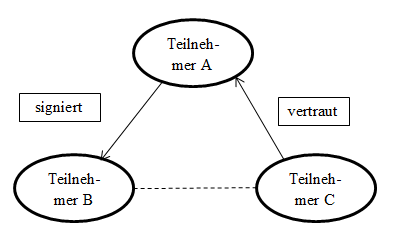
\includegraphics[width=0.4\textwidth]{images/WOT.png}
	\end{center}
	%\caption[Web of Trust Vertrauensmodell]{Web of Trust Vertrauensmodell\footnotemark}
	In Anlehnung an: \footcite[S. 120]{Ertel2012}
Teilnehmer C möchte Teilnehmer B eine verschlüsselte Nachricht schicken. Dazu besorgt er sich zunächst das Zertifikat von Teilnehmer B. Dieser wurde zuvor von Teilnehmer A signiert. Da Teilnehmer C Teilnehmer A vertraut, beschafft sich Teilnehmer C den öffentlichen Schlüssel von Teilnehmer A und verifiziert mit damit das Zertifikat von Teilnehmer B. Ist die Verifizierung erfolgreich, so kann Teilnehmer C den öffentlichen Schlüssel von Teilnehmer B vertrauen.

Bei diesem Modell wird zwischen zwei Arten des Vertrauens unterschieden. Einerseits existiert das Vertrauen in eine Person bzw. dessen Signatur. Andererseits besteht ein Vertrauen in einen signierten Schlüssel eines Dritten, der von einer vertrauensvollen Person signiert wurde. Beide Arten des Vertrauens können unabhängig voneinander existieren.
	\chapter{Sicherheitsniveaus}
	
	
		In den nachfolgenden Kapiteln dieser Arbeit werden verschiedene Möglichkeiten der Verschlüsselung von E-Mail Kommunikation vorgestellt und jeweils passende Sicherheitsniveaus zugeordnet. %das eher so ein Einleitungs-Einsatz
		
		Dabei erfolgt diese Zuordnung mit dem Ziel, einen optimalen Ausgleich zwischen Notwendigkeit und Aufwand der Verschlüsselung von E-Mails zu erhalten.
		\medskip\\
		
		%, sodass der Nutzer nach der Ermittlung eines geeigneten Sicherheitsniveaus eine aus Sicht der Autoren geeignete Verschlüsselungsmethode ermitteln kann.
	
	
		%Das nachfolgende Kapitel geht auf verschiedene Sicherheitsbedürfnisse eines Nutzers ein. 
		
		Gerade im Hinblick auf den Grad der Verschlüsselung bei der E-Mail Kommunikation ist es wichtig sich darüber bewusst zu werden, wie sensibel die Information ist, die man versenden möchte. Denn jede Verschlüsselung ist mit einem bestimmten Aufwand verbunden und folglich ist abzuwägen, welcher Verschlüsselungsaufwand dem Nutzer die zu versendende Information wert ist. 
		\medskip\\
		
		%Beispielsweise ist aus Sicht der Autoren der potentielle Schaden gering, wenn eine E-Card zu den Weihnachtsfeiertagen an den nicht rechtmäßigen Empfänger gerät, sodass für die Versendung einer solchen Information der Grad der Verschlüsselung niedrig und somit der Aufwand niedrig ausfällt. Dahingegen ist der potentielle Schaden größer, wenn es sich bei der versendeten Information um beispielsweise die eigenen Kontodaten handelt, was wiederum bedeutet, dass der Nutzer bereit ist einen höheren Aufwand zu betreiben, um diese Inhalte auf eine sichere Art und Weise via E-Mail zu übermitteln.
	
	
		%Das Sicherheitsbedürfnis einer jeden Person kann unterschiedlich stark ausgeprägt sein. 
		Der Wert einer Information ist durch das eigene Sicherheitsbedürfnis geprägt, welches jedoch von Person zu Person in unterschiedlicher Form ausgeprägt ist.
		
		Daher ist es den Autoren nicht möglich, eine allgemein gültige Auflistung aller möglichen Szenarien der E-Mail Kommunikation bereitzustellen, aus welcher die Teilnehmer der Zielgruppe lediglich das richtige Szenario heraussuchen müssen und dadurch den optimalen Grad der Verschlüsselung erhalten. 
		
		Stattdessen wird in Abbildung \ref{img:sicherheitsniveaus} eine Übersicht präsentiert, die es dem Nutzer erlaubt auf Basis seines eigenen Sicherheitsbedürfnisses und mit Hilfe festgelegter Kriterien für die Übermittlung einer ganz bestimmten Information ein geeignetes Sicherheitsniveau zu bestimmen. 
		\medskip\\
		
		
		%In den nachfolgenden Kapiteln dieser Arbeit werden verschiedene Möglichkeiten der Verschlüsselung von E-Mail Kommunikation vorgestellt und jeweils passenden Sicherheitsniveaus zugeordnet. %das eher so ein Einleitungs-Einsatz
		%Dabei erfolgt diese Zuordnung mit dem Ziel, einen optimalen Ausgleich zwischen Notwendigkeit und Aufwand der Verschlüsselung von E-Mails zu erhalten, sodass der Nutzer nach der Ermittlung eines geeigneten Sicherheitsniveaus eine aus Sicht der Autoren geeignete Verschlüsselungsmethode ermitteln kann.
	
		%Wäre nice wenn die Abbildung eine Tabelle ist, weil eine Abbildung für eine Tabelle ist irgendwie komisch :D (Pascal)
		%Auch viel Sicht der Autoren, ich würde das zur Einleitung einmal allgmein sagen statt hier 3 Mal im Absatz. So bei der Abgrenzung / Zielsetzung / einleitung. Generell ein sehr Einleitungslastiger Abschnitt.
		
		Die Abbildung \ref{img:sicherheitsniveaus} stellt im Tabellenkopf vier verschiedene Sicherheitsniveaus dar: \textit{Streng Vertraulich, Vertraulich, Privat und Öffentlich}. Dabei nimmt das Sicherheitsbedürfnis sowie der Verschlüsselungsaufwand von Streng Vertraulich bis Öffentlich ab.
		
		In der ersten Spalte sind verschiedene Merkmale aufgelistet, welche es dem Nutzer ermöglichen sollen, 
		%für eine ganz bestimmte Information 
		ein geeignetes Sicherheitsniveau zu bestimmen.
		%Nummern wären Klasse (Stufe 1-4)
		Alle weiteren Felder enthalten die Ausprägung des Merkmals innerhalb des jeweiligen Sicherheitsniveaus.
		\medskip\\
		
	\pagebreak
%	\begin{figure}[h] %{wrapfigure}[36]{l}{1.0\textwidth}
%			%\begin{center}
%		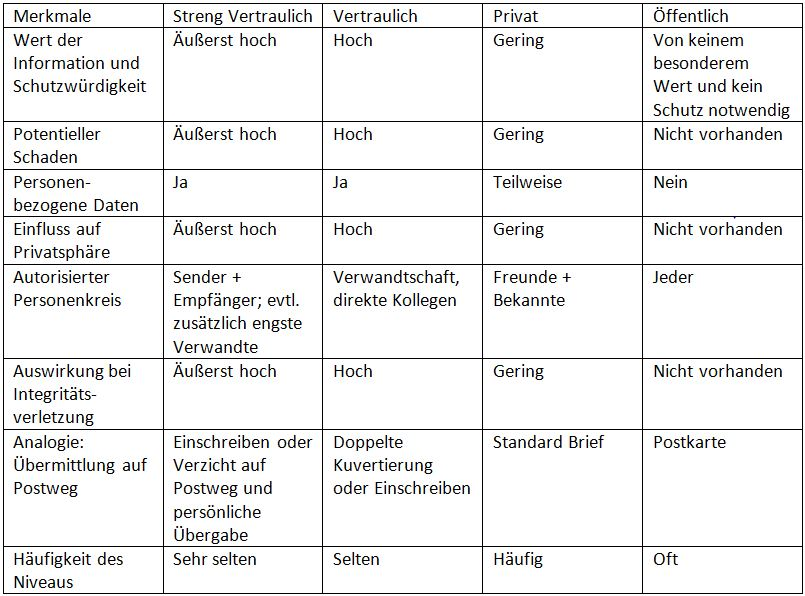
\includegraphics[width=16cm]{images/sicherheitsniveaus.jpg}
%			%\end{center}
%		\caption {Sicherheitsniveaus} %Bildunterschrift, erstes Argument ist für Abbildungsverzeichnis ohne Fußnote; \footnotemark ist ein Platzhalter für die Fußnote
%		\label{img:sicherheitsniveaus} %für Bezüge auf diese Abbildung
%	\end{figure} %wrapfigure}

	\begin{table}
		\small
		\centering
		\begin{tabularx}{\textwidth}{|>{\raggedright\arraybackslash}X|>{\raggedright\arraybackslash}X|>{\raggedright\arraybackslash}X|>{\raggedright\arraybackslash}X|>{\raggedright\arraybackslash}X|} 
			\hline Stufe & \multicolumn{1}{c|}{\textbf{4}} & \multicolumn{1}{c|}{\textbf{3}} & \multicolumn{1}{c|}{\textbf{2}} & \multicolumn{1}{c|}{\textbf{1}} \\
			  & \multicolumn{1}{c|}{\textbf{Streng Vertraulich}} & \multicolumn{1}{c|}{\textbf{Vertraulich}} & \multicolumn{1}{c|}{\textbf{Privat}} & \multicolumn{1}{c|}{\textbf{Öffentlich}} \\ 
			\hline Wert der Information, Schutzwürdigkeit & Äußerst hoch & Hoch & Gering & kein hoher Wert; kein Schutz notwendig \\ 
			\hline Personenbezogene Daten & Ja & Ja & Teilweise & Nein \\ 
			\hline Einfluss auf Privatsphäre & Äußerst hoch & Hoch & Gering & Nicht vorhanden \\ 
			\hline Autorisierter Personenkreis & Sender + Empfänger; evtl. zusätzlich engste Verwandte & Verwandtschaft & Freunde + Bekannte & Jeder \\ 
			\hline Auswirkung bei Integritätsverletzung & Äußerst hoch & Hoch & Gering & Nicht vorhanden \\
			\hline Analogie: Übermittlung Postweg & Einschreiben oder Verzicht auf Postweg und persönliche Übergabe & Doppelte Kuvertierung oder Einschreiben & Standard Brief & Postkarte \\
			\hline Häufigkeit des Niveaus & Sehr selten & Selten & Häufig & Oft \\  
			\hline
		\end{tabularx} 
		\caption{Sicherheitsniveaus}
	\end{table}
		
		Der Wert der Information und deren Schutzwürdigkeit beschreiben, wie wertvoll die zu versendende E-Mail für einen nicht rechtmäßigen Empfänger ist und welche Notwendigkeit des Schutzes daraus folgt.
		
		Der potentielle Schaden stellt das Ausmaß dar, welches eintritt für den Fall, dass die E-Mail durch 
		%unberechtigte 
		Dritte (klassische Angreifer sowie der E-Mail Provider) gelesen wird. Dieser Schaden kann verschiedener Art sein. Zum Beispiel können daraus rechtliche Konsequenzen erfolgen, es kann zu einem finanziellen Verlust führen oder mit einer Schädigung des Images des Senders einhergehen \footcite[Vgl.][]{Reinhausen GmbH, S. 6}. Aus dem potentiellen Schaden lässt sich außerdem gut der Einfluss auf die eigene Privatsphäre ableiten.
		
		
		%Habe aus Einzahl mal mehrzahl gemacht. Unberechtigte Dritte ist schwierig weil der Mailprovider ist ja quasi Berechtigt, jedenfalls stellt er das (glaub ich) zumindest in den AGBs klar. Würde nur "Dritte" sagen oder? Dazu müsste man noch klarstellen wer Dritte sind, oder verweisen (Klassische Angreifer oder Provider, Bots)
		Das Merkmal \textit{Personenbezogene Daten} besagt, dass die zu versendende Information personenbezogene Daten enthält und daher grundsätzlich das Sicherheitsniveau \textit{Vertraulich} zu wählen ist\footcite[Vgl.][]{TSE}.	In Abhängigkeit von der Ausprägung der anderen Merkmale, kann als resultierendes Sicherheitsniveau auch \textit{Streng Vertraulich} oder \textit{Privat} ermittelt werden.
		
		
		%Evtl die Beschreibungen mehr gleidern, in Absätzen oder Bullets? Weil so mitten im Text ist allg. der Text so als "Batzen" schwer zu lesen, und man kann sich auch nicht eben man die Beschreibung zur Tabelle 'heraussuchen'
		Der Autorisierte Personenkreis ist eine weitere Eigenschaft anhand derer der Nutzer ein passendes Sicherheitsniveau bestimmen kann. Grundsätzlich gilt: je wertvoller die Information, desto geringer ist der Personenkreis, der Einblick in die zu versendende E-Mail erhalten darf \footcite[Vgl.][]{TSE}. Daraus folgt, dass eine streng vertrauliche Nachricht ausschließlich zwischen dem Sender und dem Empfänger ausgetauscht wird und in der Regel keine weitere Person über den Inhalt erfahren darf. Eine Ausnahme an dieser Stelle sind allenfalls engste Verwandte. Dahingegen ist für eine Nachricht, deren Inhalt prinzipiell jedermann erfahren darf, das Sicherheitsniveau \textit{Öffentlich} zu wählen\footcite[Vgl.][]{Reinhausen GmbH, S. 10}.
		
		
		%Nachfolgend: Hier ist eindeutig ein Cut, aber deutlicher würde ich mir wünschen, eine section o.ä. wäre doch fast angebracht wenn jetzt die Auswirkungen kommen
		Die \textit{Auswirkung bei Integritätsverletzung} beschreibt das eingetretene Ausmaß, wenn die E-Mail in die Hände eines Angreifers gelangt ist.
		
		
		Eine weitere Möglichkeit ein geeignetes Sicherheitsniveau zu ermitteln ist die Überlegung, wie der Inhalt der E-Mail auf dem Postweg versandt werden würde. Für eine streng vertrauliche Information würde ein Einschreiben gewählt werden oder gänzlich auf den Postweg verzichtet und stattdessen die Nachricht persönlich überbracht werden. Dahingegen ist für Information, die ohne Bedenken  auf einer Postkarte übermittelt werden können, das Sicherheitsniveau \textit{Öffentlich} zu wählen 
		
		
		Das letzte Merkmal beschreibt das Aufkommen der einzelnen Sicherheitsniveaus. Streng vertrauliche Informationen sind sehr selten und am häufigsten werden öffentliche Nachrichten ausgetauscht \footcite[Vgl.][]{TSE}.
		\medskip\\
	%Auch wieder Cut Bsp: Anwenwedungsfälle als Section? dann Stufe 1-4 und die Fälle dazu? Das ist jetzt ein riesen Case, der unheimnlich kreativ ist und toll beschrieben. Eventuell kann es für ne wissenschaftl. Arbeit auch weniger sein nach dem Motto "Versicherungsschaden am Wagen. Bilder und Kontodaten per E-Mail an Versicherung senden: Streng vertraulich" Sowas hätte mir persönlich gereicht, und dazu vll noch ein Beispiel wie das mit den Patientendaten mit Röntgenbildern (auch streng vertraulich). Und zusätzlich noch ein paar cases zu den unteren stufen. Weihnachtsbild für die Familie mit Gesichtern : Vertraulich. Weihnachts E-Card von Webseite ohne Gesichter Öffentlich. Irgendwie sowas. Das soltlen wir besprechen am Freitag
	
		Anhand des nachfolgenden Beispiels soll der Umgang mit der Abbildung \ref{img:sicherheitsniveaus} verdeutlicht werden. Hierbei ist zu erwähnen, dass das resultierende Sicherheitsniveau auf Basis des beschriebenen Sicherheitsbedürfnisses ermittelt wurde und für die gleiche Information bei anderen Nutzern unterschiedlich ausfallen kann:
		\medskip\\
		
		Herr Meier war vor kurzem in einen Auffahrunfall verwickelt, den ein unachtsamer Autofahrer verursacht hatte. Daraufhin brachte Herr Meier sein Fahrzeug in die Werkstatt und ließ ein Gutachten des Schadens erstellen. Dieses Gutachten möchte er nun zusammen mit seinen Kontodaten via E-Mail an die Versicherung des Unfallverursachers senden. 
		
		Der Wert dieser Information ist hoch, denn einerseits sind die Kontodaten in der Nachricht vorhanden. Andererseits ist in dem Gutachten Herr Meiers Anschrift angegeben und es lässt sich aus den Fotos und der Schadenshöhe des Gutachtens ableiten, dass Herr Meier einen Luxuswagen besitzt. Daraus wiederum lassen Rückschlüsse auf seine finanzielle Situation schließen. Der potentielle Schaden, der sich daraus ergibt, ist hoch bis äußerst hoch. Denn bei ausreichender krimineller Energie können nicht nur die Kontodaten missbraucht werden, sondern mit Hilfe der Anschrift kann der Wohnsitz von Herrn Meier ausgekundschaftet und beispielsweise bei seiner Abwesenheit in sein Anwesen eingebrochen werden. 
		
		Die Anschrift stellt personenbezogene Daten dar und ermöglicht einen hohen Einfluss auf die Privatsphäre von Herrn Meier.
		Der Autorisierte Personenkreis für diese Nachricht beschränkt sich auf den Sender (Herr Meier), den Empfänger (die Versicherung) sowie auf seine Frau und auf die Werkstatt, die das Gutachten erstellt hat. Seinen Freunden und Kollegen hat Herr Meier zwar auch von dem Unfall erzählt. Allerdings wissen diese keine genaueren Details hinsichtlich des Schadens und dessen Höhe.
		
		Hätte die Versicherung den E-Mail Service nicht angegeben, so würde Herr Meier die Unterlagen des Gutachtens mit einem Standard-Brief versenden. Die Kontodaten würde er mittels Einschreiben verschicken.
		\medskip\\
		
		Somit kann als Resultat für dieses Beispiel unter dem beschriebenen Sicherheitsbedürfnis ein Sicherheitsniveau von \textit{Vertraulich} ermittelt werden. Welches Verschlüsselungsverfahren konkret für dieses Sicherheitsniveau anzuwenden ist, wird in den nachfolgenden Kapiteln beschrieben.
		
	\chapter{Gefahren und Schwachstellen}
		\label{chap:gefahren}
		\section{Informationsgewinnung durch Provider}
\textsl{
warum ist E-Mail oft Kostenlos?\\
Welchen Sinn hat das für die Provider?\\
Welche Bots lassen die Provider über unsere Kommunikation laufen?\\
Wie mächtig sind Meta-Daten?\\
\\
\\
Überleitung... Neben den weniger gerichteten (Kein Angriff?) Maßnahmen der Informationsgewinnung aus E-Mail-Kommunikation gibt es auch klassische Angriffsmethoden Dritter.\\
\\
Internetquellen, die durch Literatur idealerweise belegt wird:\\
\begin{itemize}
\item \href{http://www.netzdurchblick.de/emails.html}{netzdurchblick.de}
\item \href{https://www.eleven.de/aktuelle-pressemitteilungen.428/items/eleven-warnt-die-5-groessten-gefahren-fuer-e-mail-nutzer.html}{eleven.de}
\item \href{https://www.bsi-fuer-buerger.de/BSIFB/DE/SicherheitImNetz/OnlineBanking/GefahrenUndSicherheitsrisiken/gefahren_sicherheitsrisiken_node.html}{BSI}
\end{itemize}
Diese Quellen dienen auch zur Übersicht. Belegt werden sollten diese noch durch Literatur, die ggf. zu suchen ist!}
		 
		\section{Angriffsarten}
			\subsection{MITM - Man in the Middle}
			\label{sec:mitm}
			\subsection{Umleitungsangriffe}
			\label{sec:cache_poison}
			Umleitungsangriffe werden mit dem sogenannten \ac{DNS} Cache Poisoning durchgeführt.
			Bei diesem Angriff wird sich die Schwachstelle zu nutze gemacht, dass ältere oder falsch konfigurierte \ac{DNS}-Server auch nicht angeforderte Records in ihren Cache schreiben.
			Ein Angreifer kann dies dazu nutzen im Cache eines \ac{DNS}-Servers mithilfe von gefälschten Paketen falsche Zuordnungen von Domainnamen zu \ac{IP}-Adressen zu hinterlegen.
			Ein Opfer, das die Auflösung des Domainnamens jetzt vom kompromittierten Server anfordert, wird auf den Server des Angreifers umgeleitet.
			\subsection{Drive-By-Angriffe}
\textsl{(eleven.de)}
			\subsection{Phishing}
\textsl{Auch Spear Phising (eleven.de)}
			\subsection{Malware-E-Mails}
\textsl{Auch: Lokalisierte Angriffe (eleven.de)}
			\subsection{Spam}
\textsl{Auch: Event-Spam (eleven.de)}

		\section{Schwachstellen}
			\subsection{Zertifikatsaussteller}
			\label{sec:zertifikatsaussteller}
\textsl{AUTHENTIZITÄT (DANE-Artikel)
200 Aussteller (z.T. keine eigenen Private Keys der User) CAs können nachlässig werden. Angreifern können somit gültiges Zertifikat für einen Host erstellen dessen Besucher das Ziel sind.}
			\subsection{Zertifikatsprüfung}
			\label{sec:zertifikatspruefung}
\textsl{AUTHENTIZITÄT (DANE-Artikel)
Ideal wäre: Alle Serverzertifikate der gesamten Komunikationskette zu prüfen. In der Praxis jedoch kein sog. "Identifiziertes TLS" (Kommunikationspartner eindeutig festgestellt) In der Praxis arbeiten Server jedoch nach "Opportunistischem TLS", dass bedeutet das lediglich wichtig ist, dass die Nachricht verschlüsselt übertragen wird, egal von wem.}
			\subsection{Metadaten}
			\label{sec:metadaten}
\textsl{Quellen:
\href{http://www.spiegel.de/netzwelt/netzpolitik/google-urteil-eugh-entscheidung-zu-suchmaschinen-a-969302.html}{google-urteil-eugh-entscheidung-zu-suchmaschinen} \\
\href{http://www.golem.de/news/stanford-experiment-metadaten-verraten-intimste-details-des-privatlebens-1403-105253.html}{metadaten-verraten-intimste-details-des-privatlebens}\\
\href{http://www.heise.de/ct/heft/2014-4-Die-Schwaechen-der-E-Mail-und-was-dagegen-hilft-2092851.html}{Schwaechen-der-E-Mail-und-was-dagegen-hilft}}
	
	\chapter{Kryptographie}
		Die Kryptographie ist die Wissenschaftslehre, die sich mit den Verfahren sowie der Anwendung von Ver- und Entschlüsselung von Informationen befasst. Dabei bedient sie sich mathematischen Hilfsmitteln, um die Daten vor Dritten unzugänglich zu machen. In diesem Kapitel werden zunächst die grundlegende Funktionsweise der Verschlüsselung untersucht, die zum Verständnis der weiteren Unterkapitel notwendig sind. Anschließend werden verschiedene Verfahren beleuchtet, die eine verschlüsselte und geschützte Kommunikation ermöglichen.
		%Die Einleitung ist top, mehr Bezug zur E-Mail wäre toll, so das es essenziel für Sicherheit ist und die Basis zur Sicherstellung von sicherer Kommunikation Stufe 1-4 (Unsere niveaus) da nämlich auch öffentlich zumindest transport verschlüsselt sein sollte (wird ja auch als Standard durchgedrück (versucht) EmiG, TLS)
		\section{Grundlagen}
			\subsection{Symmetrische Verschlüsselung}
				Bei der symmetrischen Verschlüsselung wird sowohl zur Verschlüsselung und Entschlüsselung ein gemeinsamer Schlüssel verwendet. Dieser Schlüssel wird auch Shared Secret genannt. Mithilfe dieses Schlüssels und einem kryptographischen Algorithmus wird die Information des Absenders, auch als Klartext bezeichnet, verschlüsselt. Ein Algorithmus transformiert dabei einen Eingabeparameter in einen Ausgabeparameter. Im Fall eines kryptographischen Algorithmus handelt es sich um eine mathematische Vorschrift, die aus dem Klartext einen sogenannten Geheimtext berechnet. Diesen verschlüsselten Text kann der Empfänger mit dem selben Schlüssel, der zur Verschlüsselung verwendet wurde, entschlüsseln. Die folgende Abbildung zeigt das Funktionsprinzip einer symmetrischen Verschlüsselung.
				%Folgende Abbildung ist blöd, besser Wäre dann der Bezug, wenn sie drin ist wie "Die Abbildung 2 zeigt.." Also Referenzieren!
				\footnote{Kryptographie, S. 41}
				Im elektronischen Briefverkehr wirkt sich die Funktionsweise der symmetrischen Verschlüsselung nachteilig auf deren Anwendung auf. Da beide Kommunikationspartner denselben Schlüssel benötigen, muss dieser zuvor ausgehandelt und übertragen werden. Dieser Umstand stellt ein Risiko bezüglich der Vertraulichkeit dar. Jeder, der über den Schlüssel verfügt, kann auf den Inhalt der Nachricht zugreifen. Dieses Sicherheitsrisiko wird durch die asymmetrische Verschlüsselung beseitigt.
				%Wir benutzen scheinbar alle verschiedene Synonme für E-Mail Kommunikation. Elektronischer Briefverkehr klingt ganz neu für mich :D Vielleicht einigen wir uns einfach auch "E-Mail-Kommunikation"?
				%Referenzieren (Schlüsselaustausch!)	
			\subsection{Asymmetrische Verschlüsselung}
				Wie bei der symmetrischen Verschlüsselung kommt auch bei der asymmetrischen Verschlüsselung, die auch Public-Key-Kryptography genannt wird, ein kryptographischer Algorithmus zum Einsatz. Bei letzterem Verfahren wird statt eines Schlüssels ein Schlüsselpaar verwendet. Dieser besteht aus einem öffentlichen und einem privaten Schlüssel, die mathematisch zusammenhängen. Jeder, der verschlüsselte Nachrichten empfangen möchte, verfügt über ein solches Schlüsselpaar. Der private Schlüssel wird niemals bekanntgegeben, wohingegen der öffentliche Schlüssel jedem zugänglich gemacht werden kann. Obwohl die Schlüssel zusammenhängen, kann aus der Kenntnis des öffentlichen Schlüssels nicht auf den privaten Schlüssel geschlossen werden. Möchte die Nutzerin Alice bspw. mit diesem Verfahren eine verschlüsselte Mail an Bob versenden, so besorgt sie sich zunächst den öffentlichen Schlüssel von Bob. Damit verschlüsselt sie ihre Nachricht und schickt diese an Bob, der die Nachricht mit seinem privaten Schlüssel entschlüsseln kann. Die Abbildung verdeutlicht noch einmal die Funktionsweise der Public-Key-Verschlüsselung
				\footnote{Kryptographie, S. 177}
				Mit diesem Verfahren wurde das Sicherheitsrisiko der symmetrischen Verschlüsselung behoben, da der öffentliche Schlüssel zum Verschlüsseln jedem bekannt sein darf. Zur Entschlüsselung wird der dazugehörige private Schlüssel benötigt, der im Besitz des Empfängers ist und niemals veröffentlicht wird.
				Ein Sicherheitsrisiko ergibt sich jedoch aus der Tatsache, dass ein Dritter die Übertragung des öffentlichen Schlüssels von Bob abfangen und sich somit als Bob ausgeben kann, indem er seinen öffentlichen Schlüssel publiziert. In diesem sogenannten Man-In-The-Middle-Szenario kann der Dritte nun alle vermeintlich an Bob verschlüsselten Nachrichten lesen, da diese mit seinem öffentlichen Schlüssel verschlüsselt worden sind.
				Dies wird durch digitale Signaturen sichergestellt, deren Konzept im nächsten Kapitel näher untersucht wird.
			\subsection{Digitale Signaturen}\label{chp: Signatur}	
				Digitale Signaturen bieten die Möglichkeit, die menschliche Unterschrift in der digitalen Welt abzubilden. Um dies zu garantieren, müssen folgende Bedingungen eingehalten werden:
				\footnote{Kryptographie S. 202}
				\begin{itemize}
					\item Sie darf nicht zu fälschen sein.
					\item Ihre Echtzeit muss überprüfbar sein
					\item Sie darf nicht unbemerkt von einem Dokument zum anderen übertragen werden können.
					\item Das dazugehörende Dokument darf nicht unbemerkt verändert werden können.
				\end{itemize}
				Diese Voraussetzungen dienen dazu, die Authentizität des Absenders sowie die Integrität der Daten zu gewährleisten. Dazu wird das asymmetrische Verschlüsselungsverfahren genutzt. Dabei verschlüsselt der Absender seine Nachricht mit seinem privaten Schlüssel. Dieser Vorgang wird als \textit{signieren} bezeichnet. Die resultierende verschlüsselte Nachricht ist die digitale Signatur. Zusammen mit der ursprünglichen Nachricht wird die Signatur zum Empfänger geschickt. Dieser kann nun die Authentizität der Nachricht überprüfen, indem er die Signatur mit dem öffentlichen Schlüssel des Absenders entschlüsselt. Stimmt die entschlüsselte Nachricht mit der originalen Nachricht überein, so kann er sicher sein, dass die Nachricht von dem Absender stammt, da nur mit dessen privatem Schlüssel die Nachricht verschlüsselt sein konnte. Zusätzlich ist damit garantiert, dass die Nachricht vollständig und ungeändert beim Absender angekommen ist.
				
				Beim Signieren wird in der Regel aufgrund des Rechenaufwandes für lange Nachrichten nicht die gesamt Nachricht verschlüsselt, sondern ein sogenannter Hashwert der Nachricht. Hashwerte sind eine Zeichenfolge mit einer bestimmten Länge, die durch eine mathematische Einweg-Hashfunktion generiert werden. Diese Funktionen haben einen Eingabeparameter und berechnen daraus den erwähnten Hashwert. Aus der Kenntis des Hashwertes und der Funktion lässt sich der Eingabeparameter nicht ableiten. Dadurch, dass zu jedem Eingabeparameter nur ein Hashwert existiert, bleibt die Eigenschaft der Integrität erhalten.
	
			\subsection{Zertifikate}\label{chp: zertifikate}
				Bei den bisher genannten Verfahren wurde davon ausgegangen, dass der öffentliche Schlüssel wirklich dem Kommunikationspartner gehört. Die Verlässlichkeit des öffentlichen Schlüssels ist durch Szenarien wie dem Man-In-The-Middle-Angriff nicht immer garantiert. Um dies zu erreichen, werden Zertifikate benutzt.
				%Garantieren Zertifikate alleine das MITM-Attacks nicht mehr möglich sind?
				Ein Zertifikat ist ein elektronisches Dokument, das einer Person zugeordnet werden kann. Dieses Dokument enthält neben den persönlichen und weiteren Informationen des Inhabers dessen öffentlichen Schlüssel. Außerdem enthält ein Zertifikat eine Signatur über all den genannten Angaben. Das Signieren wird dabei meist von einer vertrauenswürdigen Instanz durchgeführt, die auch \ac{CA} oder Zertifizierungsstelle genannt wird.
				%Kann das nur EINER Person zugeordnet werden oder können das auch mehrere sein, oder Dienste? :)
				Möchte Alice Bob nun eine verschlüsselte Nachricht schicken, so besorgt sich Alice zunächst Bobs Zertifikat, auf dem sich dessen öffentlicher Schlüssel befindet. Um zu prüfen, ob dieser Schlüssel tatsächlich zu Bob gehört, verifiziert sie nun sein Zertifikat, indem sie die Signatur mit dem öffentlichen Schlüssel der \ac{CA} entschlüsselt. Stimmen beide Schlüssel überein, kann sie davon ausgehen, dass dieser Schlüssel tatsächlich Bob gehört.
				Das Sicherheitsrisiko bezüglich der Verlässlichkeit des öffentlichen Schlüssels der Zertifizierungsstelle wird so gelöst, indem ein Zertifikat über den öffentlichen Schlüssel erstellt wird, das von der CA selbst signiert wurde. Dieses Zertifikat wird als self-signed bezeichnet.
	
		\section{Public Key Infrastruktur}
			%Problem
			In Kapitel \ref*{chp: zertifikate} Zertifikate wurde die Definition und die Funktionsweise von Zertifikaten betrachtet. Allerdings ist der Austausch selbiger nicht ohne weiteres möglich. Denn dafür müssen sich die beiden Kommunikationspartner "kennen und einen sicheren Weg für den Austausch finden" \footcite{BSI}.\medskip\\
			
			%Idee
			An dieser Stelle setzt die so genannte \ac{PKI} an, die eine Vertrauenskette darstellt und den Austausch von Zertifikaten zweier Kommunikationspartner erleichtern soll.
			\medskip\\
			
					
			%Umsetzung
			Bei der \ac{PKI} handelt es sich um eine Hierarchie von Zertifikaten, die aus verschiedenen Elementen besteht. Auf der obersten Hierarchie Ebene steht die Wurzelinstanz, welcher auf einer oder mehrerer Unterebenen verschiedene \ac{CA} untergeordnet sind, die wiederum die Zertifikate der Endanwender signieren. \footcite[Vgl.][]{Schwenk, S.23}\medskip\\
			
			Die Wurzelinstanz wird durch die \ac{PCA} verkörpert, die  für alle vertrauenswürdig ist und ein so genanntes Wurzelzertifikat erstellt. \footcite[Vgl. ][]{ITWissen2012} 
			
			Alle weiteren Zertifikate dieser Vertrauenskette werden mit dem privaten Schlüssel des Wurzelzertifikats signiert %(vgl. Kapitel \ref{chp: Signatur} Digitale Signaturen).
			\medskip\\
						
			%Vorteile
			Dies bringt eine Reihe von Vorteilen mit sich. Zum einen können der \ac{PCA} verschieden artige \ac{CA} untergeordnet sein. Beispielsweise könnte eine \ac{CA} SSL-Zertifikate für Webserver signieren, eine weitere \ac{CA} S/MIME Zertifikate ausstellen und eine dritte \ac{CA} für die E-Mail Kommunikation zuständig sein.
			
			Zum anderen können verschiedene Sicherheitspolicies für unterschiedliche \ac{CA} hinterlegt werden. So stellt die eine \ac{CA} Zertifikate unter Voraussetzung einer gültigen E-Mail Adresse aus, wohingegen eine andere CA erst nach Vorlage eines Personalausweises ein Zertifikat signiert. \footcite[Vgl.][]{Schwenk, S.24}
			
			Ein dritter Vorteil liegt darin, dass mit Hilfe der \ac{PKI} organisatorische Strukturen, zum Beispiel die einer Unternehmung, abgebildet werden können. In solchem Falle können verschiedene CA für unterschiedliche Standorte eines Unternehmens einberufen werden, die wiederum die Zertifikate der Mitarbeiter am jeweiligen Standort signieren und deren eigenes Zertifikat durch eine übergeordnete \ac{CA} oder \ac{PCA} signiert wurde. \medskip\\
			
			Diese Vertrauenskette kann beliebig lang fortgesetzt werden, sodass zwei Kommunikationspartner sich nicht mehr gegenseitig kennen müssen um ihre Zertifikate einander auszutauschen, sondern es ausreichend ist, wenn das Zertifikat des Kommunikationspartners entlang der  \ac{PKI} von einer Instanz signiert wurde, die man selbst für vertrauenswürdig befindet. \medskip\\
			
			%Nachteile
			Jedoch liegen genau in dieser Vertrauenswürdigkeit auch die Nachteile der \ac{PKI}. Einerseits muss eine neue \ac{CA} oder \ac{PCA} erst einmal bekannt gemacht werden und auf diesem Weg vertrauen erlangen. \footcite[Vgl.][]{Schwenk, S.24}
			
			Andererseits kommt es immer wieder vor, dass \ac{CA} angegriffen werden und somit auch gefälschte Zertifikate illegal signiert werden.
				
		\section{Web of Trust}
			Das Web of Trust ist ein Vertrauensmodell, bei dem sich die Nutzer gegenseitig vertrauen und somit ein netzartiges Modell entstehen lässt. Die Grundidee ist dabei, dass die Nutzer die öffentlichen Schlüssel voneinander signieren. An einem Beispiel lässt sich das Grundprinzip dieses Modells verdeutlichen \footnote{Angewandte Kryptographie, S. 120}: Carol möchte Bob eine vertrauliche Nachricht schicken. Dazu besorgt sie sich Bobs öffentlichen Schlüssel. Zuvor hatte Alice den öffentlichen Schlüssel von Bob signiert. Da Carol Alice vertraut, beschafft sie sich die Signatur von Alice über den öffentlichen Schlüssel von Bob und entschlüsselt diesen mit Alices öffentlichem Schlüssel. Stimmen die Schlüssel überein, so kann Carol den öffentlichen Schlüssel von Bob vertrauen, weil dieser von Alice signiert wurde, der Carol vertraut. Die folgende Abbildung veranschaulicht das Funktionsprinzip:
			\footnote{S. 121, Angewandte Kryptographie}.
			%Ich denke die Abbildung ist notwendig. Aber so Steps dazu wären cool (1)..(2)..
			Bei diesem Modell wird zwischen zwei Arten des Vertrauens unterschieden. Zum einen vertraut man in einen Schlüssel, indem dieser Schlüssel durch jemand anderes, den man vertraut, signiert worden ist. Zum anderen gibt es das Vertrauen in eine Person. Diese beiden Arten sind nicht voneinander abhängig.

		\section{Schlüsselaustausch}
			Für die sichere Kommunikation ist ein sicherer Schlüsselaustausch die Ausgangsbasis um Angriffe zu verhindern. ``Hierbei ist der geschützte Austausch geheimer Schlüssel symmetrischer Kryptosysteme von Interesse.''\footcite[S. 437]{Eckert2013}
			\subsection{RSA - Rivest, Shamir und Adleman-Kryptosystem} 
				%Problem
				Beim klassischen Schlüsselaustausch werden die Sitzungsschlüssel durch den Public-Key innerhalb des Server-Zertifikat übertragen.\footcite[Vgl.][]{Boeck2013} Dies geschieht mittels \ac{RSA}-Verfahren. Verschlüsselte Kommunikation ist jedoch nur solang die Schlüssel geheim bleiben sicher. Die Gefahr beim klassischen \ac{RSA}-\ac{PKI}-Verfahren ist dass vergangene Kommunikation nachträglich zu jedem Zeitpunkt entschlüsselt werden kann, sobald Angreifer in Besitz des Private-Key sind.\medskip\\
				%Idee
			\subsection{PFS - Perfect Forward Secrecy}
				Im Gegensatz zum klassischen RSA-Schlüsselaustausch ist es sinnvoller die Sitzungsschlüssel %REFERENZ Erklären was Sitzungsschlüssel sind
				zum Einen nicht mehr zu übertragen und zum Anderen unabhängig voneinander ständig neu zu generieren und bei Terminierung zu löschen. Realisiert wird dies durch die Protokoll-Eigenschaft Forward Secrecy, die im Kryptographischen Fachjargon auch \ac{PFS}\footcite[Vgl.][]{Boeck2013} genannt wird. Die ``Anforderung an die Verfahren und Protokolle zur Schlüsselerneuerung besteht darin dafür zu sorgen, dass die Kenntnis eines Schlüssels, also dessen Aufdeckung, nicht dazu führt, dass damit auch vorherige und nachfolgende Schlüssel direkt aufdeckbar sind.''\footcite[S. 439]{Eckert2013} Wie notwendig \ac{PFS} geworden ist zeigen die jüngsten Ereignisse im Zusammenhang mit dem OpenSSL-Bug "Heartbleed", mit dem es sehr einfach war Private Schlüssel von Server auszulesen.\footcite[Vgl. ][]{Zhu2014} \medskip\\
				%Umsetzung
				Das \ac{DHE} Verfahren ermöglicht dabei als Basis die Aushandlung eines Sitzungsschlüssels bei dem die Kommunikationspartner verschiedene Nachrichten senden und sich auf einen Sitzungsschlüssel einigen können, ohne diesen je übertragen zu haben. Dieser Schlüssel ist auch nur für die aktuelle Verbindung gültig und wird anschließend gelöscht. Der Public-Key des Servers wird weiterhin übertragen, jedoch nur um den Schlüsselaustausch zu signieren. ``Abgeschlossene Sitzungen können somit im Nachhinein nicht mehr entschlüsselt werden.''\footcite[Vgl. ][]{Schulz2014} Die Verschlüsselungsverfahren \ac{TLS/SSL} und IPsec beherrschen bereits \ac{PFS}.\medskip\\
				%Vorteile
				Aufgezeichnete verschlüsselte Daten können somit bei Besitz des privaten Schlüssels nicht entschlüsselt werden. Zudem wird einfaches Belauschen einer aktiven Verbindung deutlich erschwert, denn es müsste die gesamte Kommunikation mit einem gezieltem \ac{MITM}-Angriff\ref{sec:mitm} manipuliert werden. Für diese Problematik gibt es wiederum moderne Ansätze wie DANE (Vgl. Kapitel \ref{sec:dane}), die in Kombination mit \ac{PFS} aktuell bei der Verschlüsselung von Verbindungen höchsten Sicherheitsansprüchen entsprechen, indem zusätzlich die Authentizität der Kommunikation gewährleistet wird.\medskip\\
				%Nachteile
				Nachteile gibt es lediglich bei der Verwendung des bereits überholten, und seit Jahren als geknackt bekannte \ac{DHE}-Verfahren, denn dabei verzögert sich zusätzlich der Verbindungsaufbau. Die Schlüssellänge ist Minimum 1024 Bit, und längere Schlüssel mit 2048 oder 4096 Bit sind dabei nicht sicherer.\footcite[Vgl.][]{Boeck2013} Der moderne Nachfolger mit elliptischen Kurven \ac{ECDH} gilt aktuell als sicher und benötigt dabei weniger als 1024 Bit und verzögert den Verbindungsaufbau nur unweigerlich.\medskip\\
				%Grenzen
				Obwohl es Forward Secrecy bereits seit 1999 im \ac{TLS} Standard 1.0\footcite[Vgl.][]{Boeck2013} vorgesehen ist und somit essenzieller Bestandteil von Verschlüsselung ist, hat sich \ac{PFS} noch nicht als Standard durchgesetzt.\footcite{SSLLabs} Dies liegt zum einen an den Webservern. Mit einem Apache Webserver ist nur eine Moduluslänge von 1024 Bit vorgesehen. Beim Einsatz von \ac{DHE} würden Provider damit ihre Server daher unsicher betreiben. Zum Anderen sind es auf Client-Seite die Browser die \ac{DHE} bzw. \ac{ECDH} lange Zeit ignoriert haben. Der Internet Explorer verschlüsselte nur nach DSS, wobei der de-facto Standard für Verschlüsselung bereits \ac{RSA} war. Opera unterstützte lediglich das überholte \ac{DHE}-Verfahren und Safari priorisiert Forward Secrecy niedrig und bevorzugt bei gegebener Option sogar die unverschlüsselte Kommunikation. Lediglich Firefox und Chrome unterstützen \ac{PFS} in vollem Umfang.\medskip\\
				%Browser prüfen und mit eigenen Quellen versehen
				Für die E-Mail Kommunikation ist \ac{PFS} essenziell für die Befriedigung hoher Sicherheitsbedürfnisse. Um die dazugehörigen Sicherheitsniveaus abzudecken müssen E-Mail-Server Forward Secrecy unterstützen. Im August 2013 war \ac{PFS} nur sporadisch verbreitet in der E-Mail-Kommunikationslandschaft.\footcite[Vgl. ][]{Schulz2014} Mittlerweile wird von vielen E-Mail-Providern auch \ac{PFS} angewandt. Die Umsetzung erfolgt jedoch noch zu zögerlich, wenn man die Tatsache betrachtet, dass \ac{PFS} im Zusammenhang mit Heartbleed der letzte Funken Hoffnung für betroffene Nutzer war, das zumindest vergangene Kommunikation nicht entschlüsselt werden kann.\footcite[Vgl.][]{Zhu2014}
		
		\section{Informationsverschlüsselung}
			Für hohe Sicherheitsanforderungen entscheidend ist die Vertraulichkeit der Daten. Hierfür gilt es die Authentizität und Integrität einer E-Mail sicherzustellen. Die Methode zur Umsetzung dieser Sicherheitsanforderungen ist die verschlüsselte Kommunikation zwischen zwei Endpunkten. In der E-Mail-Kommunikation wird dies mit sog. Ende-zu-Ende-Verschlüsselung (englisch \ac{E2EE}) und den Diensten S/MIME und \ac{PGP} realisiert die im Nachgang beleuchtet werden.
			Es gibt mittlerweile verschiedene Möglichkeiten \ac{E2EE} umzusetzen. Im Grunde müssen durch die Nutzer jedoch Einstellungen in den E-Mailprogrammen wie Thunderbird, Outlook oder Mail.app vorgenommen werden oder zusätzliche Software installiert werden. Demzufolge besteht ein erhöhter Einrichtungsaufwand für die Nutzer zur Sicherstellung der Vertraulichkeit und um in Sicherheitsniveaus der Grade 3 oder 4 zu kommunizieren.\medskip
			Erste E-Mail-Provider gehen zum Teil eigene Wege wenn es um die Gestaltung von benutzerfreundlicher \ac{E2EE} geht. Google bspw. arbeitet an einer Erweiterung im eigenen Chrome Browser um mittels OpenPGP zu verschlüsseln.\footcite[Vgl.][]{Somogyi2013}. Aber auch kleinere Anbieter sind an der Umsetzung für ihre Webmailer\footcite[Vgl.][]{Posteo2013} und somit \ac{E2EE} deutlich benutzerfreundlicher zu machen. 
			
			\subsection{PGP - Pretty Good Privacy}
				Die Softwarefamilie \acl{PGP} stellt ``...Dienste zur digitalen Signatur und zur Verschlüsselung von Nachrichten...''\footcite{Mueller2011} zur Verfügung und ist damit für die Vertraulichkeit der Informationen verantwortlich.
				Die größte Schwierigkeit beim Austausch von Schlüsselinformationen für \ac{E2EE} ist der für Privatanwender unbequeme Weg die öffentlichen Schlüssel auszutauschen. Dies muss noch manuell mit Hilfe von Software erfolgen und ist daher noch nicht Standard heutiger E-Mail-Kommunikation. 
				Es gibt zwar die Möglichkeit private Schlüssel durch Dienste\footnote{Bspw. iMessage von Apple für Instant Messaging} zu verteilen, jedoch ist diese Methode umstritten. Sie bietet zwar Ende-zu-Ende Verschlüsselung, jedoch ist der eigentliche Sinn des privaten Schlüssels verfehlt, wenn der Dienst bzw. Provider diesen für den Nutzer bestimmt und auf den eigenen Server zwischenspeichert. Der Nutzer hat keinen Einfluss auf den privaten Schlüssel und ist damit nicht Eigentümer dieses Schlüssels, der in Folge dessen kein Private Key ist. 
				Selbst vereinzelte \ac{CA}s gehen mit solcher Methodik vor\footcite{Kaps2014}, und untergraben damit die Sicherheit des ganzen \ac{CA}-Modell. \medskip\\
				Mit PGP werden kryptographische Dienste bereitgestellt die unter anderem Dateiverschlüsselung, Schlüssel-Recovery und das Signieren von Dokumenten umfassen.
				Ab Version 5.0 wird in PGP neben \ac{RSA} auch \ac{DHE} zum Austausch symmetrischer Schlüssel und eine symmetrische Blockchiffre für die Mailverschlüsselung verwendet. Die Integrität der Daten ``... und Authentizität wird durch die Verwendung von \ac{SHA}-1 und \ac{MD5} als Hashfunktionen bzw. als \ac{MAC}s sichergestellt.''\footcite[][S.823]{Eckert2013}\medskip
				Für das Format zur Verschlüsselung und Signierung von Daten nach \ac{PGP} 5 bietet OpenPGP einen Standard nach \acs{RFC} 4880. Ein entsprechendes Programm zur Implementierung dieses Standards ist \ac{GPG} für gängige E-Mail-Clients um die Verschlüsselung und den Schlüsselaustausch so benutzerfreundlich wie möglich zu gestalten. Zu Berücksichtigen ist hierbei der Faktor das Private Keys nur lokal gespeichert und durch sichere Passphrasen geschützt sind.
				
			\subsection{S/MIME - Secure / Multipurpose Internet Mail Extensions}
				
		\section{Transportwegverschlüsselung}
			Das \ac{SSL}-Protokoll wurde zunächst durch die Firma Netscape entwickelt, um die Kommunikation über \ac{HTTP}-Verbindungen abzusichern.\footcite[Vgl.][S. 796]{Eckert2013} \ac{SSL} kann auf der Sitzungs- und Präsentationsschicht des \ac{OSI}-Referenzmodells angesiedelt werden und setzt meist auf dem \ac{TCP} auf. Es hat die Aufgabe den darüber liegenden Schichten die Möglichkeit für eine authentifizierte, integritätsgeschützte und verschlüsselte Kommunikation zu geben.\footcite[Vgl.][S. 799 ff.]{Eckert2013}
			Die Version \ac{SSL} 3.0 hat sich mittlerweile als de facto Standard im Internet durchgesetzt und wird von allen gängigen Browsern unterstützt.\\
		
			\begin{wrapfigure}{r}{0.4\textwidth} %wrapfigure ist eine Umgebung, in dem eine Abbildung von TExt umgeben werden kann; {r} steht für rechts, {l} geht auch; zweites Argument ist die Breite des "Einfügekastens"
				\begin{center}
					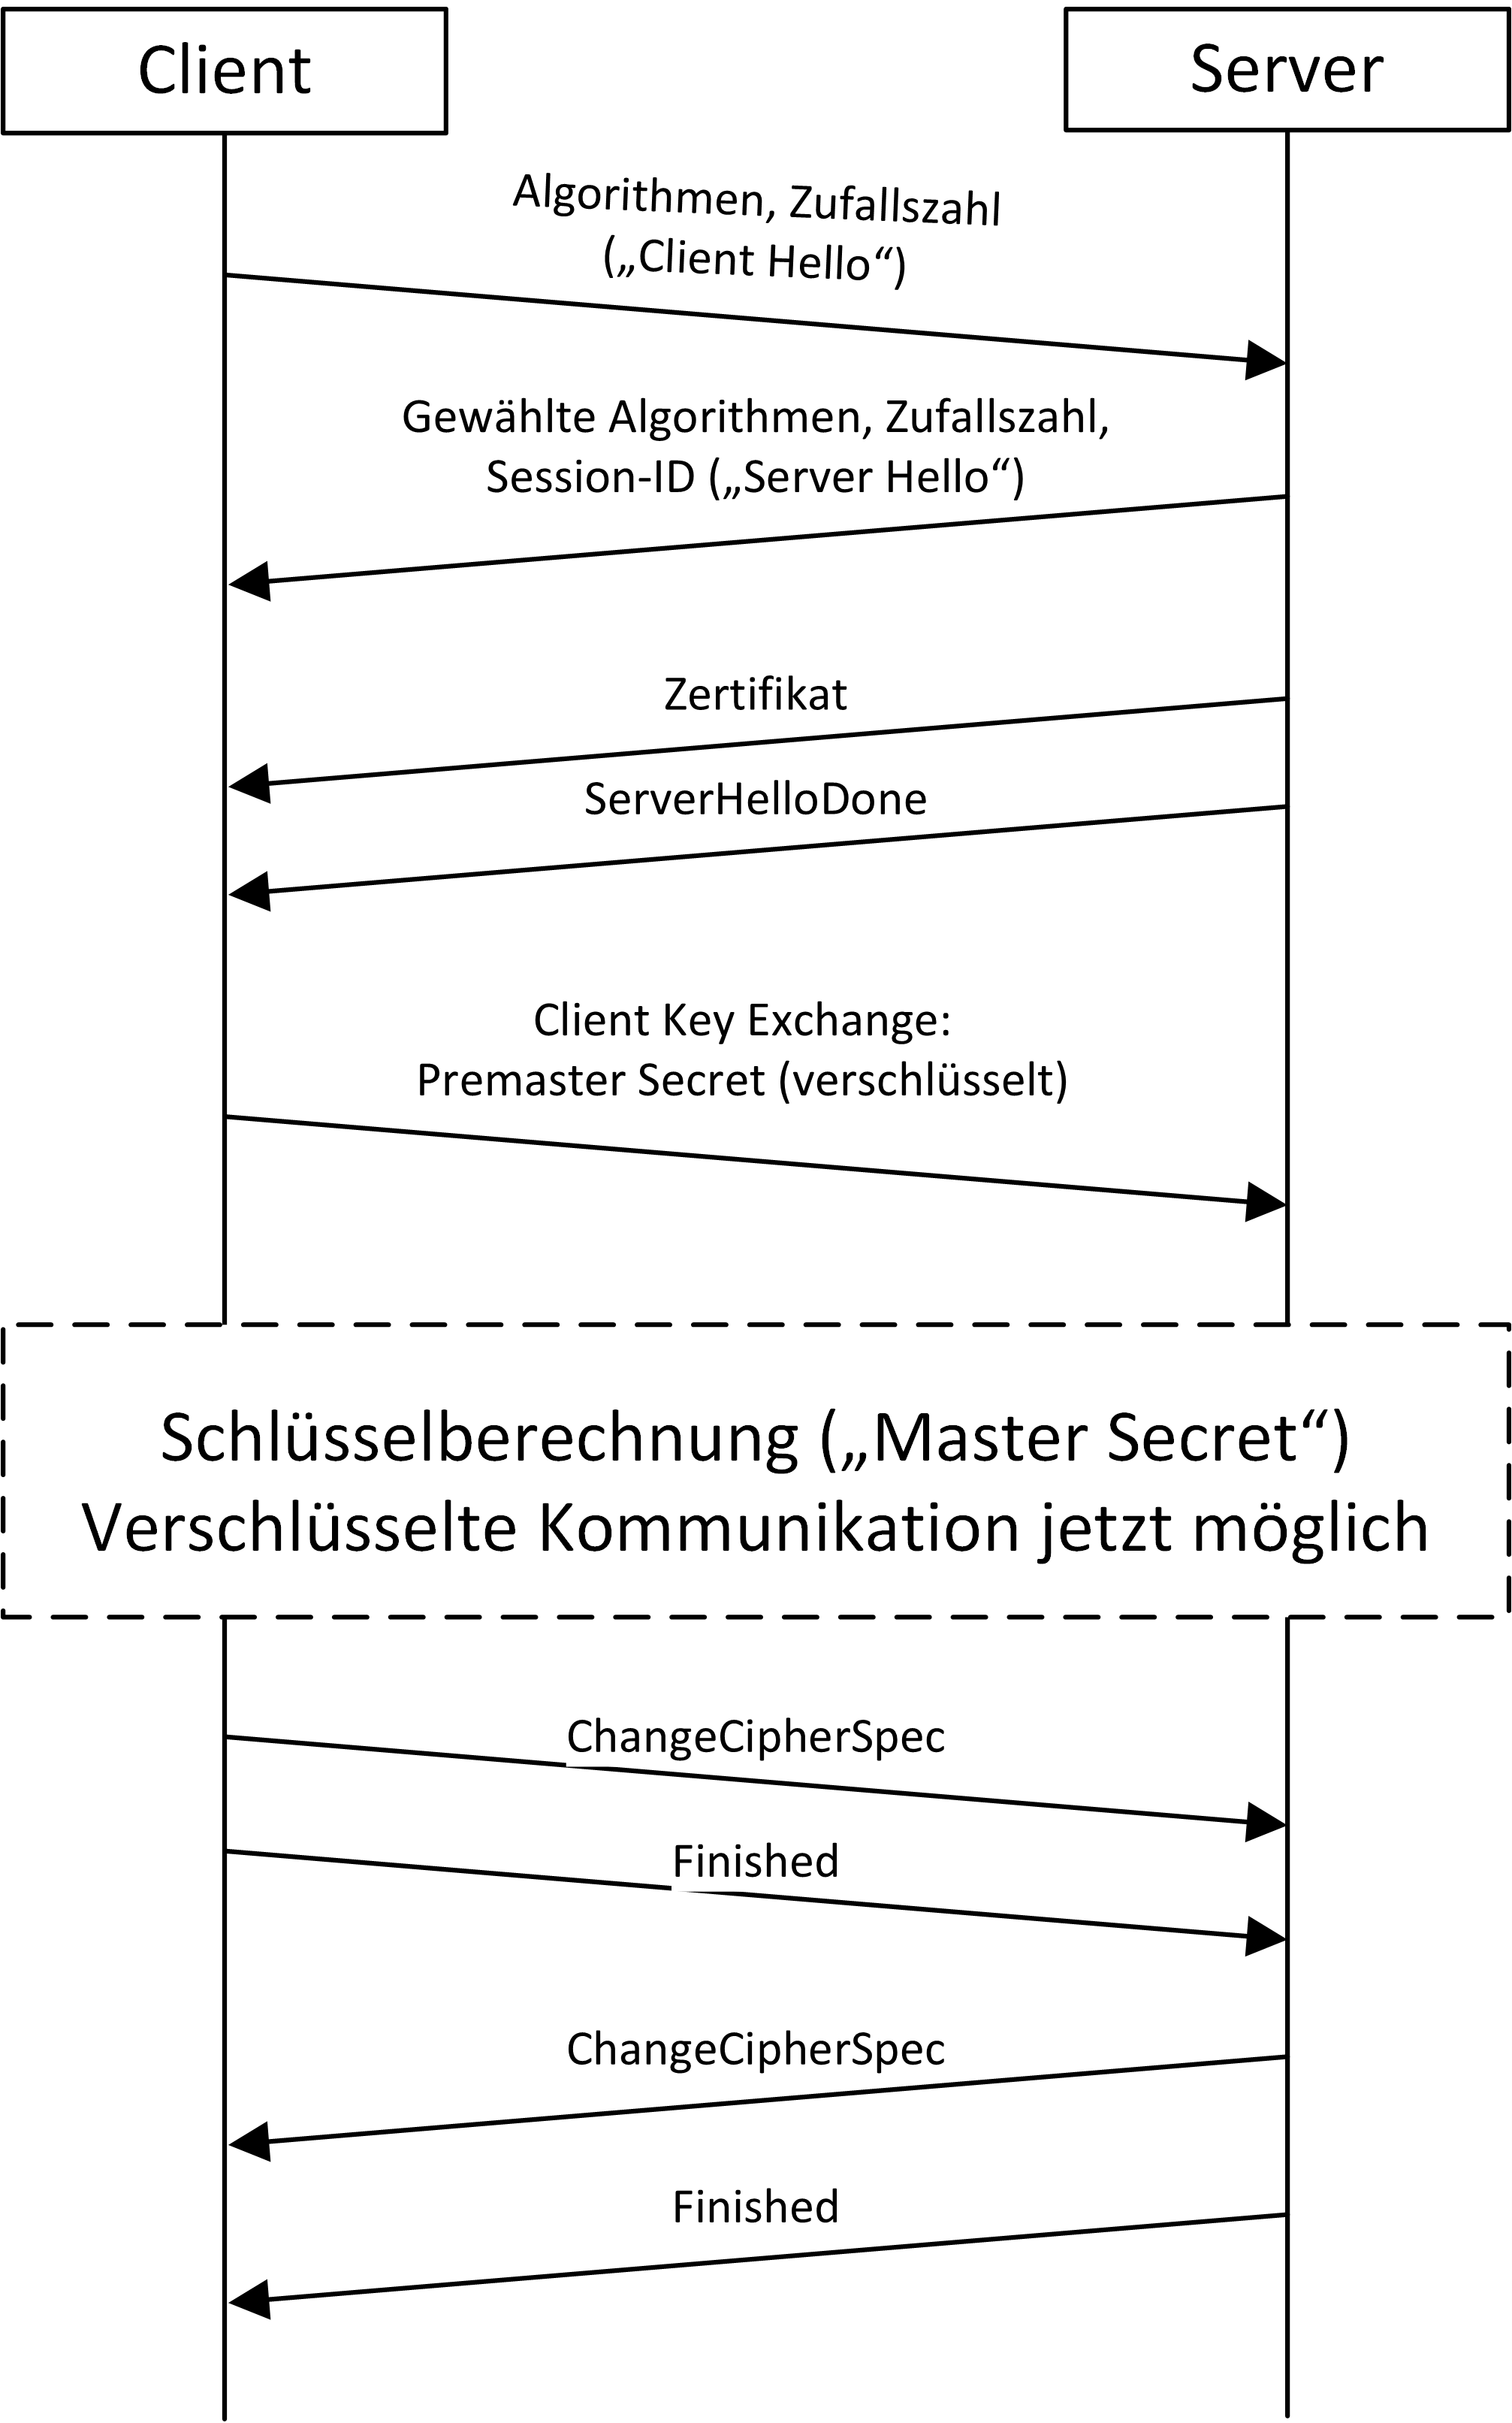
\includegraphics[width=0.4\textwidth]{images/MSC_Transport.png}
				\end{center}
				\caption[Handshake-Protokoll mit RSA]{Handshake-Protokoll mit RSA\footnotemark} %Bildunterschrift, erstes Argument ist für Abbildungsverzeichnis ohne Fußnote; \footnotemark ist ein Platzhalter für die Fußnote
				\label{img:MSC_Transport} %für Bezüge auf diese Abbildung
			\end{wrapfigure}\footnotetext{\cite[In Anlehnung an][S. 170]{Sorge2013}} 
			Das \ac{TLS}-Protokoll kann als Weiterentwicklung von \ac{SSL} 3.0 angesehen werden und liegt aktuell in der Version 1.2 vor.
			Da beide Protokolle in ihren Kernkonzepten übereinstimmen werden sie häufig synonym verwandt. Da \ac{TLS} jedoch eine Weiterentwicklung von \ac{SSL} ist, werden dort einige Erweiterungen eingeführt sowie unsichere Verfahren zur Berechnung von \ac{MAC}-Werten durch neuere Varianten ersetzt.\\
		
			%\begin{figure}
			%	\begin{minipage}{0.5\textwidth}
			%		\centering
			%		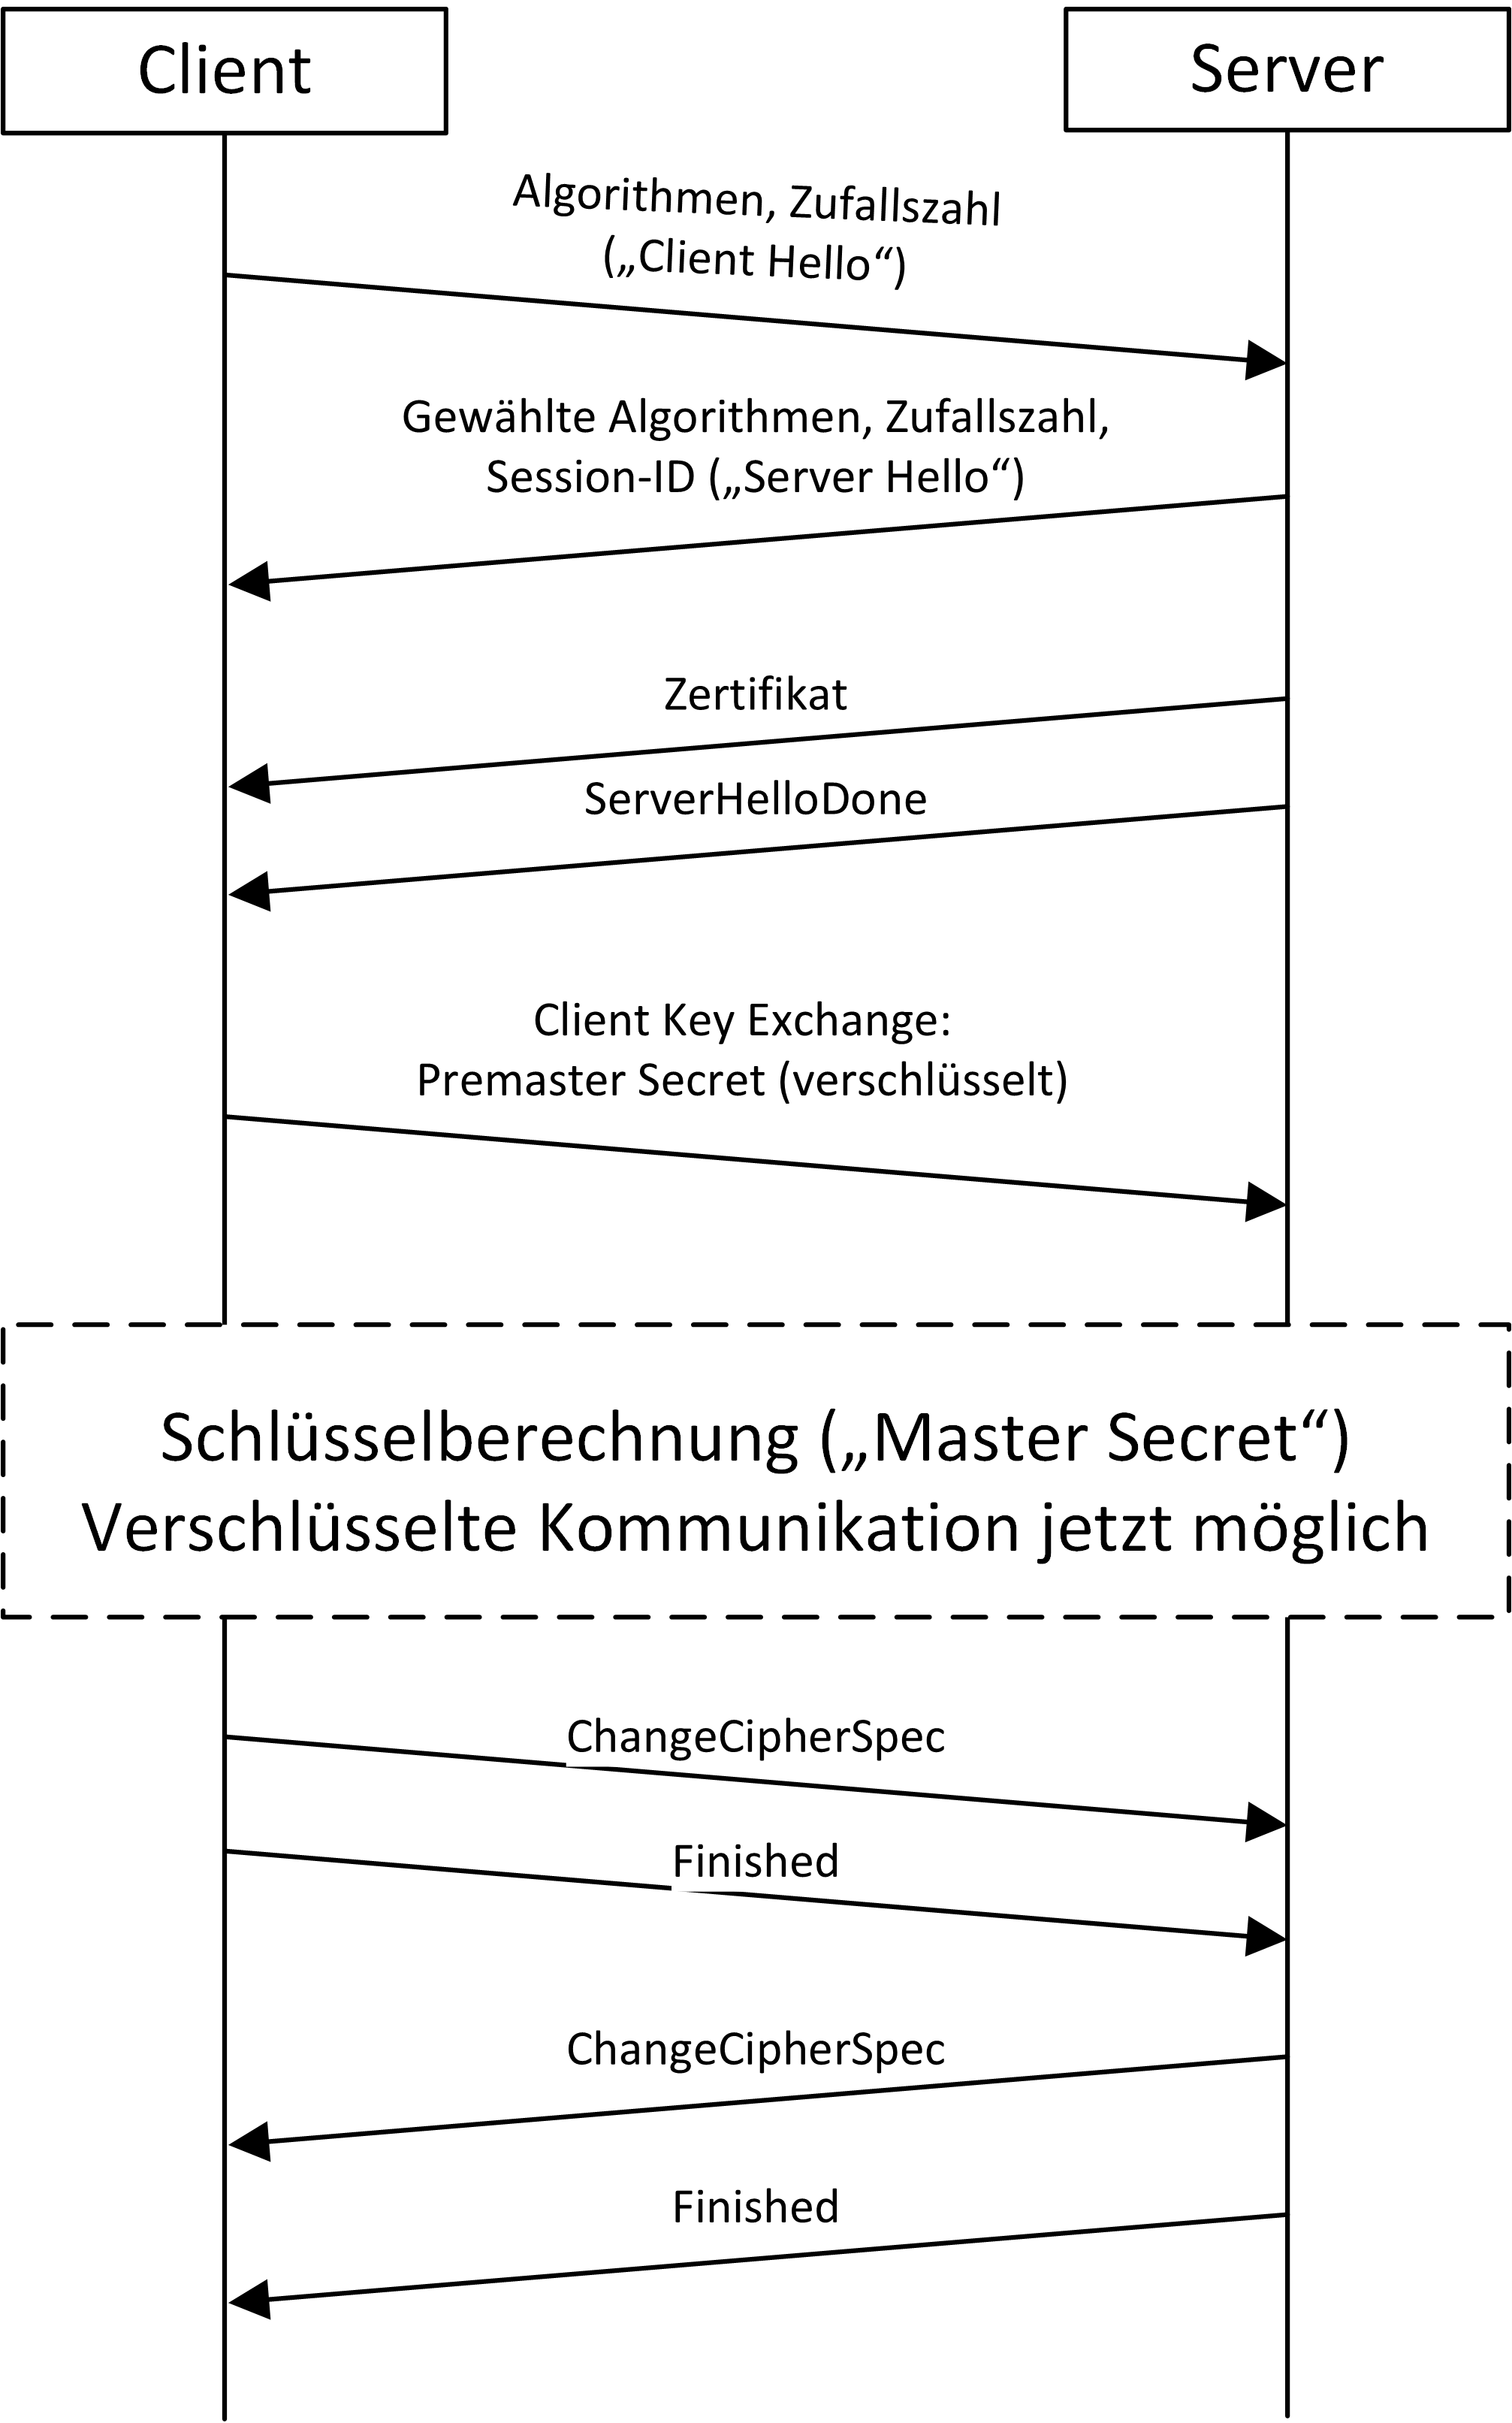
\includegraphics[width=0.45\textwidth]{images/MSC_Transport.png}
			%		\caption[Handshake-Protokoll mit RSA]{Handshake-Protokoll mit \ac{RSA}\footcite[In Anlehnung an:][S. 170]{Sorge2013}}
			%	\end{minipage}
			%\end{figure}
			
			Beide Protokolle bestehen aus mehreren Schichten bzw. Unterprotokollen wobei das Record- und das Handshakeprotokoll von besonderer Bedeutung sind. 
			Das Record-Protokoll ist für die Fragmentierung, Authentifizierung mittels \ac{MAC} und Verschlüsselung der zu übertragenden Daten zuständig. 
			Mittels des Handshakeprotokolls werden Sitzungen zwischen den Kommunikationspartnern hergestellt. 
			Dies bedeutet, dass die Kommunikationspartner durch den Austausch von Zertifikaten authentifiziert werden können und alle Informationen, die zur Berechnung des Shared Secret für die symmetrische Verschlüsselung der Daten benötigt werden, ausgetauscht werden. 
			Abbildung \ref{img:MSC_Transport} verdeutlicht den schematischen Ablauf eines solchen Sitzungsaufbaus unter Verwendung von \ac{RSA} für den Schlüsselaustausch.\\
			
			Durch die flexible Gestaltung des Handshake-Protokolls wird gleichzeitig auch die Komplexität von \ac{TLS/SSL} stark erhöht. 
			Dies hat zur Folge, dass durch die hohe Komplexität nicht mit Sicherheit alle Schwachstellen beim Design des Protokolls entfernt werden konnten. 
			Außerdem ist zu bedenken, dass \ac{TLS/SSL} aufgrund seiner weiten Verbreitung ein lohnendes Ziel für Angriffe ist. Die Sicherheit des Protokolls hängt dabei stark von den genutzten kryptologischen Methoden ab. 
			Außerdem ist zu beachten, dass es sich, aufgrund der Ansiedlung des Protokolls unterhalb der Anwendungsschicht, nur um eine Verschlüsselung der transportierten Nutzdaten auf dem Transportweg handelt. 
			Die Daten werden am Kommunikationsendpunkt entschlüsselt und anschließend an die entsprechende Anwendung weitergereicht.
			Dies bedeutet für die Anwendung im Bereich des E-Mailversands, dass die Nachrichten weiterhin im Klartext auf den Servern der Mailprovider vorliegen und von jedem, der berechtigten oder unberechtigten Zugang zu diesen erhält, ausgelesen werden können.
			Im Sinne der definierten Sicherheitsniveaus ist die \ac{SSL}-Verschlüsselung daher auf der zweitniedrigsten Stufe anzusiedeln, da das Mitlesen der versandten Mails zwar erschwert, aber nicht unmöglich gemacht wird.\\
			
			%\acp erzeugt den Plural des Akronyms bzw. hängt ein "s" an
			Auch die Authentifizierung der Kommunikationspartner mittels Zertifikaten weißt dieselben Schwachstellen durch die Vertrauensbeziehung zu bekannten \acp{CA}, die unzureichend gesichert sind, auf.  
			%Hier noch ein kurzer Abschnitt zu Metadaten mit Bezug auf die Schwachstellen (sec:metadaten)
	\chapter{DNS - Domain Name System}
	\label{chap:dns}
		Das \ac{DNS} ist ein wichtiger Dienst im Internet, da er dafür zuständig ist, gut merkbare Domainnamen in \ac{IP}-Adressen, und umgekehrt, aufzulösen.
		Um diese Auflösung bewerkstelligen zu können ist \ac{DNS} in einer Baumstruktur aufgebaut. 
		Wie in der Abbildung\footnote{Abb. in Anlehnung an Sorge S. 180 einbinden} veranschaulicht, ist auf der obersten Ebene der Knoten "root" zu finden.
		Dies ist sozusagen die Wurzel des \ac{DNS} und hier finden sich auch die Root-Server des \ac{DNS}
		Auf der nächsten Ebene kommen die \ac{TLD}, anschließend folgen die Second-Level-Domains und zum Aufbau einer gängigen \ac{URL} für \ac{HTTP} fehlt noch eine weitere Ebene, die den Hostnamen enthält.
		Soll ein Domainnamen aufgelöst werden, so fragt der Host zunächst einen Root-Server.
		Dieser sendet ihm die Adresse des für die entsprechende \ac{TLD} zuständigen Nameservers mit, an die der Client eine erneute Anfrage stellt.
		Auch der Nameserver der \ac{TLD} verweist den Client an für die Second-Level-Domain zuständigen Nameserver.
		Auf diese Weise kann der Client den dargestellten Baum traversieren, bis er die gewünschte Information erhält.
		Die für diese Auskünfte benötigten Datensätze werden in sogenannten \ac{DNS}-Records abgelegt.
		Das Problem ist hierbei, dass allein mit den \ac{DNS}-Records nicht die Authentizität des Absenders (vgl. \ref{sec:cache_poison}) und damit auch nicht die Integrität der Daten sicher gestellt werden kann.
		Dies wird jedoch für eine sichere E-Mailkommunikation benötigt, da auch die Domainnamen der Mailserver einer Zone über \ac{DNS}-Records vom Typ \glqq MX\grqq aufgelöst werden.
%		Dies wird beim sogenannten \ac{DNS} Cache Poisoning %Das unter "E-Mail-Kommunikation-Gefahren" einbauen.
%	 	ausgenutzt und der Cache eines \ac{DNS}-Servers manipuliert.
%		Zumeist werden dabei mittels gefälschter Pakete an einen \ac{DNS}-Server falsche Zuordnungen von Domainnamen auf \ac{IP}-Adressen hinterlegt, um ein Opfer auf den Server des Angreifers umzuleiten.
		\section{DNSSEC - Domain Name System Security Extensions}
		\label{sec:dnssec}
			Bei \ac{DNSSEC} handelt es sich um eine Sicherheitserweiterung des \ac{DNS}.
			Sie beruht auf der Einführung weiterer \ac{DNS}-Records.
			Unter anderem gibt es einen Recordtyp, der einen öffentlichen Schlüssel enthält und einen weiteren, der die Signatur eines Ressource Records enthält.
			Ein autoritativer Nameserver kann eine Zone an einen anderen Nameserver delegieren und hält dann einen Verweis auf den entsprechenden Nameserver vor.
			Dadurch gibt es pro Zone des \ac{DNS} maximal einen \ac{ZSK} mit dem die Ressource Records dieser Zone signiert werden, dies ist jedoch nicht zwingend notwendig.
			Mithilfe dieser Schlüssel und Signaturen kann nun eine Zertifikatskette aufgebaut werden.
%			Ein Schwachpunkt dabei ist, dass mindestens ein öffentlicher Schlüssel, der als \ac{KSK} fungiert und den \ac{ZSK} einer Zone signiert, auf einem sicheren Weg zum Client kommen muss.
%			Daher wird dieser Schlüssel auch als Secure Entry Point bezeichnet.
			Ein Kritikpunkt an \ac{DNSSEC} ist die hohe Komplexität des Systems, die durch den Aufbau der Zertifikatsketten und dem aufwändigen Austausch der Schlüssel auf Zonenebene entsteht.
			Diese ist jedoch der benötigten Kompatibilität mit bestehenden Systemen geschuldet und momentan alternativlos.\footcite[Vgl.][S. 195]{Sorge2013}
			\ac{DNSSEC} ist im Prinzip eine eigene \ac{PKI} deren Hauptschlüssel Root DNSSEC Key die Non-Profit-Organisation \ac{ICANN} verwaltet.\footcite{Koetter2014}. Der "Hauptschlüssel und damit die \ac{DNSSEC}-\ac{PKI} [kann] als vertrauenswürdig [angesehen werden]."\footcite{Koetter2014} Entscheidender Grund hierfür sind die 21 \ac{TCR} die an der Erstellung des root key und der Signierungsprozesse partizipieren.
	
		\section{DANE - DNS-based Authentication of Named Entities}
		\label{sec:dane}
			Die Basis für die Applikation \ac{DANE} stellt \ac{DNSSEC} und soll dabei die Schwachstellen von \ac{TLS} beim Verschlüsseln des Datentransport entfernen. Denn die Authentizität der verwendeten Zertifikate kann nicht immer gewährleistet werden, und somit besteht die Gefahr der kompromittierten Daten durch \ac{MITM}-Angriffe oder \ac{DNS}-Cache-Poisoning.
			Die Schwachstellen der Zertifikatsprüfung und -aussteller (Vgl. Kapitel \ref{sec:zertifikatsaussteller} und \ref{sec:zertifikatspruefung}) werden mittels \ac{DANE} eliminiert, denn es werden damit nicht mehr mehrere CA-Stellen benötigt. Lediglich das DNS der Empfängerdomain benennt das gültige Zertifikat. Die somit  veröffentlichte Prüfsumme aus dem Server-Zertifikat des Ziels kann durch den sendenden Server zutreffend identifiziert werden.\medskip\\
			Die Aufgabe von \ac{DANE} besteht darin \ac{TLS}-Zertifikate über das \ac{DNS} automatisch zu verteilen und zu prüfen. Dabei ist \ac{DANE} nicht auf E-Mail Protokolle beschränkt sondern ist vielmehr für sämtlichen verschlüsselten Datenverkehr einsetzbar.
			Serverbetreiber tragen den Hash (Fingerabdruck) vom eigenen Public Key in die \ac{DNS}-Zone ein damit das eigene Zertifikat prüfbar wird. Ein Sender erhält bei einer \ac{DNSSEC} gesicherten \ac{DNS}-Anfrage den passenden \ac{TLSA}-Record. Für die Zertifikatsprüfung wird anschließend aus dem empfangenen Publik Key des \ac{TLS}-Verbindungsaufbau auf dem Sender der Hash berechnet. Ist der Fingerabdruck dem Hash aus der \ac{DNS}-Abfrage identisch ist die Verbindung vertrauensvoll.
			Ein durchgängig verfizierter Transport ist allerdings nur möglich wenn alle beteiligten Mail-Server \ac{TLSA}-Records vorhalten. Wenn eine Prüfstelle keinen besitzt muss ``müssen [die Server] auf ungeprüftes \ac{TLS} zurückfallen oder gar unverschlüsselt kommunizieren''\footcite[S. 197]{Koetter2014}
			Bisher ist \ac{DNSSEC} noch kein Durchbruch gelungen. Aber die Situation für identifizierte, sichere E-Mail-Kommunikation ist dank \ac{DANE} deutlich besser, denn ``die Verwendung [...] ist u.a. schon bei \ac{IPsec}, \ac{SSH}, \ac{PGP} und \ac{S/MIME} angedacht,''\footcite[S. 196]{Koetter2014} und für \ac{HTTPS} bereits 2012 standardisiert worden. Die \ac{SMTP}-Standardisierung ist in der Finalisierungsphase. Wenn sich \ac{DANE} durchsetzt ist die Kommunikation nicht nur unter E-Mail-Verbünden wie \ac{EmiG} gewährleistet, sondern auch mit der restlichen Welt. Bisher scheitert \ac{DANE} allerdings an der Unterstützung der Browser, von denen kein gängiger \ac{DANE} ohne Add-on umsetzt.
	\chapter{E-Mail-Sicherheit in der Praxis}
		\section{Provider Vergleich}
			\subsection{Internationale Provider}
				Googlemail\\
				Hotmail\\
				Yahoo Mail
			\subsection{EmiG - E-Mail made in Germany}
\textsl{web.de, gmx.de, t-online \\
Meine Quellen:\\
\\
\begin{itemize}
\item \href{http://www.heise.de/netze/meldung/So-funktioniert-E-Mail-made-in-Germany-2188248.html}{So-funktioniert-E-Mail-made-in-Germany}\\
\item
\href{http://www.heise.de/netze/meldung/E-Mail-made-in-Germany-Vollstaendig-umgesetzt-dennoch-unzureichend-2179269.html}{E-Mail-made-in-Germany-Vollstaendig-umgesetzt-dennoch-unzureichend}\\
\item
\href{http://www.e-mail-made-in-germany.de/Verschluesselung.html}{e-mail-made-in-germany.de/Verschluesselung}\\
\item
\href{http://www.heise.de/security/meldung/30C3-E-Mail-Unsicherheit-made-in-Germany-2072758.html?wt\_mc=rss.security.beitrag.atom}{E-Mail-Unsicherheit-made-in-Germany}\\
\item
\href{http://www.heise.de/newsticker/meldung/Was-der-Beitritt-zu-E-Mail-made-in-Germany-kostet-2189578.html}{Was-der-Beitritt-zu-E-Mail-made-in-Germany-kostet} \\
\item
\href{https://mailbox.org/e-mail-made-in-germany-verhindert-systematisch-teilnahme-anderer-provider/}{e-mail-made-in-germany-verhindert-systematisch-teilnahme-anderer-provider}\\
\item
\href{http://www.heise.de/newsticker/meldung/mailbox-org-wirft-E-Mail-made-in-Germany-Blockadehaltung-vor-2191020.html}{mailbox-org-wirft-E-Mail-made-in-Germany-Blockadehaltung-vor}  \\
\end{itemize}
} 

			\subsection{Alternative Provider}
				posteo\\
				mailbox.org\\
				startmail
		\section{Nutzwertanalyse E-Mail-Provider}
			<Hier Nutzwertanalyse beschreiben und einbetten, ggf. im Anhang darauf verweisen>
	\chapter{Ausblick}
		(Trends/Fazit/Schlusswort -> proton Mail Provider vom CERN)
		(Google hat die alpha eines Plugins für Chromebrowser vorgestellt, die E2E-Verschlüsselung im Browser durchführen und vereinfachen soll -> könnte nen Hinweis wert sein) 	
		Da das Thema noch aktuell ist, und ständig weiter lebt macht es vll Sinn genau nochmal drauf aufmerksam zu machen das es nur um eine Moment-Aufnahme handelt. 		
	\chapter*{Literaturverzeichnis}
		\addcontentsline{toc}{Literaturverzeichnis}{Literaturverzeichnis}
		%Literaturverzeichnis
		\printbibliography[heading=offline,nottype=online]
		\printbibliography[heading=online,type=online]
	\chapter*{Anhang}
		\addcontentsline{toc}{Anhang}{Anhang}
\end{document}